%==============================================================================
% Autor: Marius Iustin Grossu xgross10
%==============================================================================
% kodovani: UTF-8 (zmena prikazem iconv, recode nebo cstocs)
%------------------------------------------------------------------------------
% zpracování / processing: make, make pdf, make clean
%==============================================================================
\documentclass[zadani]{fitthesis} % odevzdani do wisu a/nebo tisk s barevnými odkazy - odkazy jsou barevné
%---rm---------------
\renewcommand{\rmdefault}{lmr}%zavede Latin Modern Roman jako rm / set Latin Modern Roman as rm
%---sf---------------
\renewcommand{\sfdefault}{qhv}%zavede TeX Gyre Heros jako sf
%---tt------------
\renewcommand{\ttdefault}{lmtt}% zavede Latin Modern tt jako tt

\csdoublequotesoff



\usepackage{url}


% =======================================================================
\ifWis
\ifx\pdfoutput\undefined % nejedeme pod pdflatexem / we are not using pdflatex
\else
  \usepackage{color}
  \usepackage[unicode,colorlinks,hyperindex,plainpages=false,pdftex]{hyperref}
  \definecolor{hrcolor-ref}{RGB}{223,52,30}
  \definecolor{hrcolor-cite}{HTML}{2F8F00}
  \definecolor{hrcolor-urls}{HTML}{092EAB}
  \hypersetup{
	linkcolor=hrcolor-ref,
	citecolor=hrcolor-cite,
	filecolor=magenta,
	urlcolor=hrcolor-urls
  }
  \def\pdfBorderAttrs{/Border [0 0 0] }  % bez okrajů kolem odkazů 
  \pdfcompresslevel=9
\fi
\else % pro tisk budou odkazy, na které se dá klikat, černé 
\ifx\pdfoutput\undefined % nejedeme pod pdflatexem 
\else
  \usepackage{color}
  \usepackage[unicode,colorlinks,hyperindex,plainpages=false,pdftex,urlcolor=black,linkcolor=black,citecolor=black]{hyperref}
  \definecolor{links}{rgb}{0,0,0}
  \definecolor{anchors}{rgb}{0,0,0}
  \def\AnchorColor{anchors}
  \def\LinkColor{links}
  \def\pdfBorderAttrs{/Border [0 0 0] } % bez okrajů kolem odkazů 
  \pdfcompresslevel=9
\fi
\fi
% Řešení problému, kdy klikací odkazy na obrázky vedou za obrázek
\usepackage[all]{hypcap}

% Informace o práci/projektu
%---------------------------------------------------------------------------
\projectinfo{
  %Prace / Thesis
  project={BP},            %typ práce BP/SP/DP/DR  
  year={2022},             % rok odevzdání 
  date={29. července 2022},             % datum odevzdání 
  %Nazev prace / thesis title
  title.cs={Dolování dat v prostředí jazyka Python},  % název práce v češtině či slovenštině (dle zadání)
  title.en={Data Mining in the Python Language}, % název práce v angličtině 
  %Autor
  author.name={Marius Iustin},   % jméno autora 
  author.surname={Grossu},   % příjmení autora 
  %Ustav 
  department={UIFS}, % doplňte příslušnou zkratku dle ústavu na zadání: UPSY/UIFS/UITS/UPGM 
  % Školitel / supervisor
  supervisor.name={Vladimír},   % jméno školitele / supervisor name 
  supervisor.surname={Bartík},   % příjmení školitele / supervisor surname
  supervisor.title.p={Ing.},   %titul před jménem (nepovinné) 
  supervisor.title.a={Ph.D.},    %titul za jménem (nepovinné) 
  % Klíčová slova / keywords
  keywords.cs={získávání znalostí z databází, dolování dat, programovací jazyk Python, knihovny pro dolování dat, dolování asociačních pravidel, klasifikace, shlukování, analýza dat}, % klíčová slova v českém či slovenském jazyce 
  keywords.en={knowledge discovery from databases, data mining, Python programming language, libraries for data mining, mining association rules, Classification, Clustering, data analysis}, % klíčová slova v anglickém jazyce 
  % Abstrakt / Abstract
  abstract.cs={Tato práce se zaměřuje na problematiku získávání znalostí z databází v prostředí jazyka Python. Jejím cílem je prozkoumat možnosti dostupných knihoven pro získávání znalostí v tomto jazyce a jejich podporou pro jednotlivé metody pro řešení úloh z dané problematiky pomocí experimentů. Experimenty se zaměřují na metody pro zisk asociačních pravidel, klasifikaci a shlukování implementované v jednotlivých vybraných knihovnách. Pro každý experiment se zvolila vhodná datová sada. Výstupem této práce je porovnání vybraných knihoven a zhodnocení, která knihovna je nejvhodnější pro použití v oblasti získávání znalostí z databází.}, % abstrakt v českém či slovenském jazyce
abstract.en={This thesis is focused on the field of obtaining knowledge discovery from databases in the Python. Its aim is to explore the possibilities of available libraries for data mining in this programming language and their support for individual methods for solving problems using experiments. The experiments focus on methods for obtaining association rules, classification and clustering implemented in individual selected libraries. An appropriate data set was chosen for each experiment. The output of this work is a comparison of selected libraries and an evaluation of which library is most suitable for use in the field of knowledge discovery from databases.}, % abstrakt v anglickém jazyce
  % Prohlášení (u anglicky psané práce anglicky, u slovensky psané práce slovensky) 
  declaration={Prohlašuji, že jsem tuto bakalářskou práci vypracoval samostatně pod vedením pana Ing. Vladimíra Bartíka, Ph.D.
Uvedl jsem všechny literární prameny, publikace a další zdroje, ze kterých jsem čerpal.},
  acknowledgment={Chtěl bych poděkovat vedoucímu práce, pánovi Ing. Vladimírovi Bartíkovi, Ph.D. za odbornou pomoc, vstřícnost a rady, které mi pomohli k vyprácování této práce.},
  %faculty={FIT}, % FIT/FEKT/FSI/FA/FCH/FP/FAST/FAVU/USI/DEF
  faculty.cs={Fakulta informačních technologií}, % Fakulta v češtině - pro využití této položky výše zvolte fakultu DEF
  faculty.en={Faculty of Information Technology}, % Fakulta v angličtině - pro využití této položky výše zvolte fakultu DEF
  department.cs={}, % Ústav v češtině - pro využití této položky výše zvolte ústav DEF nebo jej zakomentujte 
  department.en={} % Ústav v angličtině - pro využití této položky výše zvolte ústav DEF nebo jej zakomentujte
}

\clubpenalty=10000
\widowpenalty=10000

% checklist
\newlist{checklist}{itemize}{1}
\setlist[checklist]{label=$\square$}

% Nechcete-li, aby se u oboustranného tisku roztahovaly mezery pro zaplnění stránky, odkomentujte následující řádek
% \raggedbottom

\begin{document}
  % Vysazeni titulnich stran
  % ----------------------------------------------
  \maketitle
  % Obsah
  % ----------------------------------------------
  \setlength{\parskip}{0pt}

  {\hypersetup{hidelinks}\tableofcontents}
  
  % Seznam obrazku a tabulek (pokud prace obsahuje velke mnozstvi obrazku, tak se to hodi)
  \ifczech
    \renewcommand\listfigurename{Seznam obrázků}
  \fi
  \ifslovak
    \renewcommand\listfigurename{Zoznam obrázkov}
  \fi
  % {\hypersetup{hidelinks}\listoffigures}
  
  \ifczech
    \renewcommand\listtablename{Seznam tabulek}
  \fi
  \ifslovak
    \renewcommand\listtablename{Zoznam tabuliek}
  \fi
  % {\hypersetup{hidelinks}\listoftables}

  \ifODSAZ
    \setlength{\parskip}{0.5\bigskipamount}
  \else
    \setlength{\parskip}{0pt}
  \fi

  % vynechani stranky v oboustrannem rezimu
  \iftwoside
    \cleardoublepage
  \fi

  % Text prace
  % ----------------------------------------------
  \ifenglish
    \input{projekt-01-kapitoly-chapters-en}
  \else
    %=========================================================================
% Autor: Marius Iustin Grossu xgross10
\chapter{Úvod}
\label{uvod}
Žijeme v době, kdy se generuje velké množství dat díky technologiím, která naše společnost disponuje. Každý den se nová data ukládají po celém světě v databázích za účelem je transformovat v prospěšnou informaci a znalost, která může být použita v komerční nebo vědecké sféře. Vzhledem k uspěchané době a velkému objemu dat, není čas se na to manuálně podívat. Proto vznikla nová odvětví z oblasti výzkumu databází, která se zabývá automatizaci těchto činností.

V současné době má datový analytik nebo inženýr k dispozici velké množství nástrojů pro automatizaci, ať už jsou komerčně nebo bezplatné. Takovým nástrojem je například vysokoúrovňový programovací jazyk Python. Zásluhou spoustě volně dostupných knihoven pro zpracování, analýzu, vizualizaci a modelování dat získává tento programovací jazyk na popularitě mezi odborníky z oblasti dolování dát. Tato práce se zaměřuje právě na dostupné knihovny pro získávání znalostí tohoto jayzka a následné porovnání a zhodnocení jejich možností.

Všeobecný teoretický úvod pro získávání znalostí z databází se nachází v kapitole \ref{ziskavani}. Vyhrazená kapitola \ref{metody} popisuje konkrétní metody pro řešení různých typu dolovacích úloh. V následující kapitole \ref{python} je představen jazyk Python a jeho dostupné knihovny a popisuje jejich vlastnosti, možnosti a podporu pro získávání znalostí. V kapitole \ref{experimenty} jsou demonstrované experimenty, které ukazují možností jednotlivých knihoven. Každý experiment představuje datovou sadu, která byla vhodná zvolena pro daný typ dolovácí úlohy, následně její implementaci v daných knihovnách a zhodnocení výsledků. Závěrečné zhodnocení jednotlivých knihoven a doporučení nejvhodnější knihovny se nachází v kapitole \ref{zhodnoceni}.

\chapter{Získávání znalostí z databází}
\label{ziskavani}
Tato kapitola se věnuje popisu problematice získávání znalostí z databází. Bude zde stručně představena teorie, která je nezbytná k pochopení dalších částí této práce.

Na úvod budou definované pojmy získávání znalostí z databází a dolování dát. Dále se představí jednotlivé kroky procesu získávání znalostí databázi. Další důležitou částí je, které druhy dat jsou vhodné pro dolování a závěr je věnován popisu typických úloh.

\section{Co je získávání znalostí z databází a dolování dát}
\label{coje}
Častokrát se pojmy získávání znalostí z databázi (v angličtině knowledge discovery in databases) a dolování dat (data mining) používají jako synonyma a proto se musí jednoznačně rozlišit. 

Formálně lze říct, že získávání znalostí z databáze je proces extrakce netriviálních, skrytých, dříve neznámých, užitečných modelů dat a vzorů z velkých objemů dat. Tyto modely a vzory následně reprezentují získané znalosti.
Dolování dat (také dolování z dat) je jedna část tohoto procesu, při které se aplikuje algoritmus pro získávání znalosti. \cite{Dunham} 

Jakákoliv operace nad daty, která porušuje nějakou z vlastnosti uvedena v definici, nepatří do této oblasti. Takovým příkladem může být obyčejné vyhledávání informaci nebo použití jednoduchých SQL příkazů, které porušují vlastnost netriviálnosti. 

Dolování dat sjednocuje v sobě techniky z různých výzkumných oblastí jako je databázová technologie, statistika, strojové učení, vysoce náročné výpočty, rozpoznávání vzoru, neuronové sítě a vizualizace dat \cite{Han}. Zároveň z praktického hlediska využívá dolování dát například bioinformatika, biznis, vzdělávací systémy, zdravotnictví, finance nebo kriminalistika \cite{Neha}. 

\section{Kroky procesu získávání znalostí}
Jak bylo zmíněno v předchozí podkapitole, získávání znalostí z databází je proces skládající se z několika kroků, které se v určitých iteracích opakují. Tento proces je znázorněn na obrázku \ref{proces}.

Jednotlivé kroky procesu jsou \cite{Han}:

\begin{enumerate}
    \item \textit{Čištění dat} -- tento krok odstraňuje šum, řeší nekonzistence dát a vypořádá se s chybějícími hodnotami v datech.
    \item \textit{Integrace dat} -- zde dochází ke sloučení dat z několika různých zdrojů. Tento krok s předchozím krokem se často provádí společně, protože vyčištěna data je potřeba někam uložit. Data se ukládají do datového skladu, jak je znázorněno na obrázku.
    \item \textit{Výběr dat} -- tento krok vybírá data, která jsou relevantní pro řešení dané analytické úlohy.
    \item \textit{Transformace dat} -- zde dochází k transformaci dát do konsolidované podoby vhodné pro dolování. Příkladem takové transformace může být agregace nebo sumarizace.
    \item \textit{Dolování dat} -- tento důležitý krok vytváří model dat tím, že extrahuje vzory z dat pomocí aplikace určitě metody a konkrétního algoritmu. 
    \item \textit{Hodnocení modelů a vzorů} -- zde cílem je identifikovat opravdu zajímavé vzory na základě mír užitečnosti.
    \item \textit{Prezentace znalostí} -- tento poslední krok má za úkol ukázat výsledky dolování uživateli využitím různých technik vizualizace a reprezentace znalostí.
\end{enumerate}

\begin{figure*}[h]\centering
  \centering
  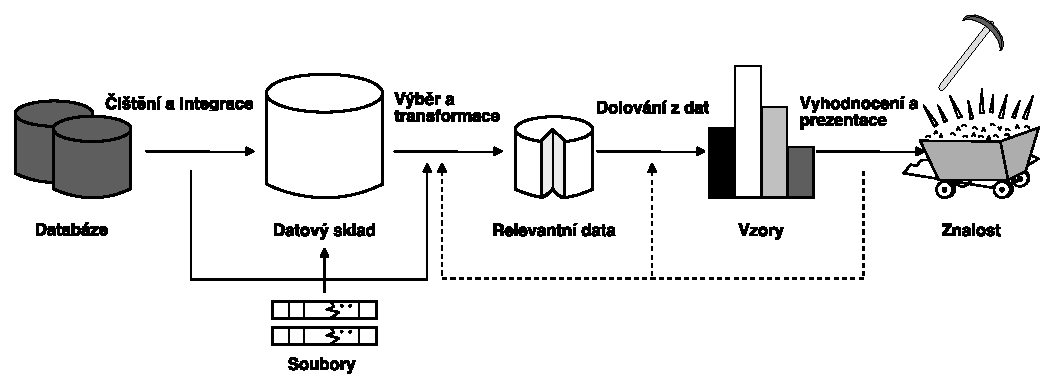
\includegraphics[width=\linewidth,height=1.7in]{obrazky/proces_dolovani.pdf}\\[1pt]
  \caption{Proces získávání znalostí (převzatý z \cite{Han})}
  \label{proces}
\end{figure*}

Kroky 1 až 4 procesu prezentován výše jsou různou formou předzpracování dat. Jádrem procesu je krok \textit{dolování dat}, při kterém může docházet k interakci s uživatelem nebo může algoritmus využít databázi znalostí, z které získá nějakou znalost o datech. Tato znalost se označuje jako \textit{doménová znalost}. Podle ní, podle výběru vstupu dolovácí úlohy, podle výběru výsledného modelu nebo znalostí, podle výběru algoritmu, podle definic hraničních hodnot a nebo způsobu vizualizace se proces získávání znalostí může lišit v různých případech \cite{Han}.

\section{Druhy dat pro dolování}
V podstatě můžeme dolovat nad jakýmkoliv informačním repozitářem, který obsahuje smysluplné údaje. Může se jednat o data které jsou persistentní uložena na nějakých úložištích nebo transientních, jakými jsou proudy dat. Nejčastějšími zdroji dat, které existují, mohou byt relační databáze, datové sklady a transakční databáze, ale jsou i jiné typy zdrojových dat, které budou zde uvedené. \cite{Han} 

\subsection*{Relační databáze}
Jak už z názvu vyplívá, hlavním prvkem tohoto typu databází je relace. Relace se skládá ze dvou částí, kterými jsou: relační schéma a instance relace. \textit{Instance relace} je tabulka, která se skládá z množiny několika záznamů. Záznam je jeden řádek tabulky, který má vždy stejný počet sloupců, které se můžou chápat jako atributy daného záznamu. Název a doménu každého sloupce určuje \textit{relační schéma}. Záznamy můžeme identifikovat pomocí primárních klíčů. Primární klíč se skládá z neprázdné množiny atributů. Tabulka musí splňovat podmínku první normální formy a ta je, že data v jednotlivých sloupcích tabulek musí být atomické. \cite{Elmasri}

K datům se typický dostaneme prostřednictvím databázových dotazů v jazyce SQL. Tím se dá získat spousta užitečných informacích, které můžou pomoct při rozhodování, ale nejde o dolování, jak bylo už bylo zmíněno v podkapitole \ref{coje}. Při dolování jde získat mnohem komplexnější informace jako trendy, modely a vzory.

Relační databáze je jedním z nejběžnějším zdrojem dat a proto se hojné využívá jako typ zdroje dat pro dolovaní.
\subsection*{Datové sklady}
Datový skald je úložiště údajů, pro které platí, že údaje pochází z různých datových zdrojů. Vzniká pomocí procesu, kde se data vyčistí, integrují, transformují, načítají a periodicky se aktualizují. Datové sklady jsou nezbytnou součástí v organizacích, které je využívají pro strategické rozhodování, a taky důležitou platformou pro získávání znalostí. \cite{Fernando}

Pro jednodušší rozhodování jsou údaje organizované okolo hlavních subjektů, například pokud bychom měli úspěšného prodejce elektroniky, který má desítky poboček po celé Evropě, tak takovými subjekty by byli zákazník, položka, dodavatel apod \cite{Han}. Data jsou též uložena z historické perspektivy, to znamená, že postihují čas, například sklad obsahuje data za posledních několik let. Další vlastnosti dat v datovém skladu je, že jsou sumarizovaná. Nejednalo by se například o jednotlivé prodeje v jednotlivých pobočkách, ale o sumární hodnoty prodeje typů položek v jednotlivých pobočkách nebo po regionech ve dnech, měsících nebo čtvrtletích. Typická práce s datovým skaldem je znázorněna na obrázku \ref{datove-sklady}.

\begin{figure*}[h]\centering
  \centering
  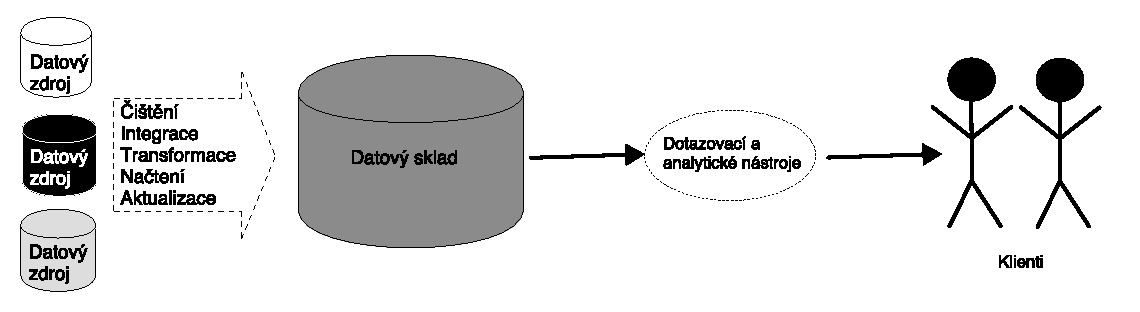
\includegraphics[width=\linewidth,height=1.7in]{obrazky/datovy-sklad-arch.pdf}\\[1pt]
  \caption{Vytvoření a využití datového skladu (převzatý z \cite{Han})}
  \label{datove-sklady}
\end{figure*}

Datový sklad jaký modelován pomocí struktury, která se nazývá \textit{multidimenzionální kostka}. 
To umožňuje poskytnout multidimenzionální pohled na data a taky tím, že data jsou agregovaná, je vhodný pro provádění OLAP (Online Analytical Processing) operací.
Díky OLAP operacím poskytuje datový sklad mnohem větší podporu pro analýzu oproti běžným produkčním databázím. Takovou multidimenzionální kostku je možné vidět na obrázku \ref{kostka}. \cite{Han}

\begin{figure*}[h]\centering
  \centering
  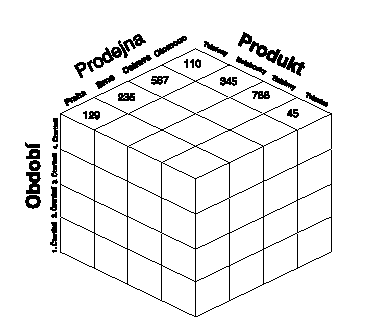
\includegraphics[width=4in,height=3.5in]{obrazky/kostka.pdf}\\[1pt]
  \caption{Multidimenzionální kostka modelující datový sklad}
  \label{kostka}
\end{figure*}

\subsection*{Transakční databáze}
Tento další druh databázi ukládá data na základě jistého druhů časově známky. Obecně lze říct, že transakční databáze je obyčejný soubor, kde každý záznam ukazuje jednu transakci. Transakce typicky obsahuje jednoznačný identifikátor transakce a seznam položek. \cite{Han}

Nejedná se tedy o klasickou transakcí z databází, ale jde o obchodní transakcí. Takovým příkladem je nákup zboží nějakým zákazníkem např. v pekárně. V takovém případě by položkami mohl být kód nebo nějaká jiná identifikace pečiv, která pekárna nabízí a jejich seznam v záznamu transakce by udával, co všechno zákazník koupil při jednom nákupu. Obvykle transakční databáze obsahují další tabulky s dodatečnými informacemi o položkách transakce. Transakční databázi je možné spatřit na obrázku \ref{trasakcni-tabulka}.

\begin{figure*}[h]\centering
  \centering
  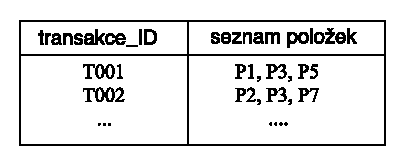
\includegraphics[width=3.5in,height=1.2in]{obrazky/db-transakce.pdf}\\[1pt]
  \caption{Transakční databáze (převzatý z \cite{Han})}
  \label{trasakcni-tabulka}
\end{figure*}

\subsection*{Další typy zdrojů dát}
Kromě častých výše uvedených příkladů, další typy zdrojů dát mohou byt následující \cite{Han}:
\begin{itemize}
    \item \textit{Web} -- velká, stále rostoucí, heterogenná databáze, která obsahuje různorodé formáty dat nabízící velký potenciál pro zisk znalostí.
    \item \textit{Textové databáze} -- databáze, která obsahuje nestrukturovaná, částečně strukturovaná textová data (HTML, JSON) nebo strukturovaná textová data (katalogy knihoven).
    \item \textit{Proudy dat} -- data produkována spojitě nebo opakovaně, která mají vlastnosti, že jejích objem je obrovský, potenciálně nekonečný a neustále se dynamický měnící. Data se neskladují neomezené. 
    \item \textit{Prostorové databáze} -- obsahují data, která vyjadřuje prostorové uspořádání. Takovým příkladem může být geografické databáze obsahující data map a objektů na nich.
    \item \textit{Multimediální databáze} -- úložiště pro obrazová data,  audio a video data. Textové databáze mohou taky spadat pod multimediálními databáze.
    \item \textit{Časově závislé databáze} -- databáze, která ukládá údaje vztahující se k času. Může se jednat například o různé typy události, které se dějou v čase.
\end{itemize}
\section{Typy dolovacích úloh}
\label{typyuloh}
Zde si představíme charakteristiku základních typu dolovacích úloh. Typem dolovacích úloh se rozumí, o jaký druh modelu dat se snažíme z dat získat. Toto probíhá v kroku dolovaní dat celého procesu. 
Prvně se představí popis konceptu/třídy, následně hledaní frekventovaných vzoru, klasifikace, predikce, shlukovaní a nakonec ostatní méně časté úlohy.
Takovým základním rozdělením typu dolovacích úloh může byt do dvou skupin \cite{Han}:

\begin{enumerate}
    \item  \textit{Deskriptivní} – jejich cil je charakterizovat všeobecné vlastnosti mezi daty. Představitel tohoto typu úloh může být například hledaní asociačných pravidel nebo shlukovaní.
    \item \textit{Prediktivní} – cílem tohoto typu je na zaklade současných dat předpovědět budoucí chovaní. Příklad tohoto typu je klasifikace nebo regrese.
\end{enumerate}

Při kroku tohoto procesu se generuje velké množství vzoru. Obvykle však se uplatňuje, že jen mala část z nich je pro koncového uživatele zajímavá. Proto před samotným popisem jednotlivých technik je vhodné si uvést nějaké kritéria, která odlišuje skutečně zajímavé vzory od nezajímavých \cite{Han}:

\begin{itemize}
    \item novost
    \item jednoduchá srozumitelnost pro člověka
    \item platnost pro nové nebo testovací data s jistým stupněm určitosti
    \item potenciální užitečnost
\end{itemize}

Tyto kritéria jsou klíčová, aby vytvořeny vzor mohl být označen za znalost.

\subsection*{Popis konceptu/třídy}
Jedná se o jeden ze základních typu dolovacích úloh. Řadí se do kategorie deskriptivních úloh. Cílem je zde poskytnout stručný, souhrnný a výstižný popis určité množiny dat. Například ve firmě prodávající elektroniku můžou byt spotřebiče rozdělené do tříd: notebooky a chytré telefony, prostory firmy mohu rozdělené do tříd: prodejny a sklady. Tyto třídy je vhodné charakterizovat popisem, který je možné získat díky jednomu z následujících způsobů \cite{Han}.

\begin{itemize}
    \item \textit{Charakterizací dat} - výsledná třída je popsána sumarizaci jejich obecných vlastností. Platí, že jednoduchým dotazem z databáze se vybírají data odpovídající třídě.
    \item \textit{Diskriminace dat} - výsledná třída je popsaná rozdíly mezi jednou nebo více třídami. Třídy, s kterým se porovnává, jsou nazývaný rozdílové.
\end{itemize}

\paragraph{Příklad 2.4.1} Charakterizace dat \newline
Může se jednat o charakterizaci zákazníků, kteří utrácí víc jak třicet tisíc korun ročně za elektroniku. Jsou to zákaznici ve věku 25 až 35 let a jsou zaměstnání v IT firmě. 

\paragraph{Příklad 2.4.2} Diskriminace dat \newline
Výsledek by porovnal různé skupiny zákazníků. Například, že 70\% zákazníků, kteří často kupují počítač jsou ve věku 20 až 35 let a mají vysokoškolské vzdělání, ale 50\% zákazníků, kteří občas kupují počítač, tak jsou buď senioři nebo mládež bez vysokoškolského vzdělání.

\subsection*{Frekventované vzory}
Jedná se o další typ dolovácí úlohy pro odhalování vztahu mezi atributy. Jak už název napovídá jsou to vzory, které se často objevují v datech. Existují mnoho typů frekventovaných vzoru: frekventované množiny, frekventované podsloupností nebo jiné struktury jako například podstromy, podgrafy apod. Typický za frekventovanou množinu označujeme množinu položek, která se spolu vyskytují často. \cite{Han}

Takovým příkladem může být nákup chytrého telefonů a obal k němu. Velmi často zákaznici kupují tyto položky v jednom nákupu. Jako příklad frekventované podsloupností může byt  série nákupu jednoho zákazníka. Zákazník si nejdřív koupit notebook, ale zjistí, že víc pracuje doma, takže následně koupí nový monitor a poslední nákup je myš a klávesnice.

Dolováním frekventaných vzorů odhalujeme zajímávé asociace a korelace. Odhalování zajímavých asociací se označuje jako \textbf{asociační analýza}. Výsledkem takové analýzy jsou \textbf{asociační pravidla}. Často bývá asociační analýza doplněna o hledání korelací mezi dvojicemi asociačních pravidel. \cite{Dunham} Tvar formátu asociačního pravidla je následující (\ref{pravidlo1}):

\begin{align}
    \textit{kupuje(X, 'chytrý telefon')}  \Rightarrow \textit{kupuje(X, 'obal')} [\textit{podpora} = 5\%, \textit{spolehlivost} = 70\%],
    \label{pravidlo1}
\end{align}

kde proměna X označuje zákazníka. Toto pravidlo nám popisuje, že zákaznici kteří si kupují nový chytrý telefon, tak mají tendenci si koupit i obal k němu ve stejném nákupu. Významnost pravidla v tomto případě nám určuje dvě míry: \textit{podpora} a  \textit{spolehlivost}. Podpora 5\% udává, že 5\% nákupu obsahuje spolu položky chytrý telefon a obal. Spolehlivost 70\% udává, že v 70\% nákupů si zákazník v případě koupě nového chytrého telefonu, koupil i obal k němu. Tyto dvě jsou nejčastěji používané míry, ale existují i další. Asociační pravidla, které nepřesáhnou minimální hranici těchto parametrů, bývají typický odstraněné.

Uvedené asociační pravidlo obsahuje jen jeden predikát, proto se nazývá \textit{jednodimenzionální asociační pravidlo}. Obecně může asociační pravidlo obsahovat víc než jeden predikát, například pravidlo (\ref{pravidlo2}):

\begin{align}
    \textit{věk(X, '15..25')} \wedge \textit{pohlaví(X, 'žena')} \Rightarrow \textit{kupuje(X, 'obal')}[\textit{podpora} = 1\%, \textit{spolehlivost} = 65\%]
    \label{pravidlo2}
\end{align}
     
obsahuje 3 predikáty: \textit{věk, pohlaví} a \textit{kupuje}. Takový pravidla se označkují jako \textit{multidimenzionální asociační pravidla}. \cite{Han}

Dolování frekventovaných vzorů, asociací a korelací má velké úplatnění v praxi. Příkladem může být hledání strategické polohy skupiny produktů v prodejně nebo doporučení dalšího vhodného filmu k shlédnutí.

\subsection*{Klasifikace a predicke}
Patří mezi prediktivní úlohy dolování dat. \textbf{Klasifikace} si dává za cíl vytvořit model, který popisuje a současně rozlišuje třídy dat. Dále je model využíván pro predikci kategorických hodnot. To znamená, že hodnoty jsou diskrétní a neuspořádané. Tím se odlišuje od \textbf{predikci}. Ta slouží k predikování numerických hodnot spojitého charakteru. Nejčastější metodou predicke je \textit{regresivní analýza}. \cite{Dunham}

\paragraph{Příklad 2.4.3} Klasifikace a predikce \newline
Manažer firmy, která prodává elektroniku chce zjistit, kteří zákaznici jsou důvěryhodní, a naopak kteří jsou rizikoví z pohledu splacení koupeného zboží. Klasifikační model, který by vznikl na základě popisných vlastnostech o zákaznících jako např. typ zaměstnání, měsíční příjem, historie splácení předešlých zboží apod, by klasifikoval, který zákazník je důvěryhodný a který ne.

Dále by manažera této firmy zajímalo, kolik by utratil zákazník ve věku od 25 do 35 let v budoucím měsíci, pokud by zlevnil veškeré zboží o 10\%. Pomocí predikce se zjistí tato neznáma numerická hodnota a manažer by nasledně zvážil, zda se vyplatí taková sleva.\newline

Kromě výše uvedeného příkladu klasifikace a predikce mají v praxi mnoho dalších úplatnění. Pomáhají například ve zdravotnictví, marketingu a všude tam, kde je potřeba něco identifikovat nebo předpovědět.
Proces klasifikace se skládá ze tří kroků: trénování/učení, testování a aplikace. Obvykle je potřeba jistým způsobem upravit zdrojová data na vstupů před započetím procesu klasifikace. Základní úpravy jsou následující \cite{Han}:

\begin{itemize}
    \item Čištění dat - odstraňování chybějících hodnot.
    \item Analýza významnosti - odstraňování atributů objektů, které jsou zpohledu klasifikace nepotřebné.
    \item Transformace dat - převod dat na jiný formát (například kategorizace nebo normalizace hodnot)
\end{itemize}

V první fázi, kdy probíhá trénování/učení, tak se analyzuje soubor dat. Tento soubor je označován jako treningová množina objektů. Pro jednotlivé objekty této množiny platí, že známe jejích třídu. Pomocí této vlastnosti je možné vytvořit klasifikační model, který dokáže prediktovat třídy neznámých objektů. Průběh fáze je ilustrovaná obrázkem \ref{faze-trenovani}. \cite{Bharati} 

\begin{figure*}[h]\centering
  \centering
  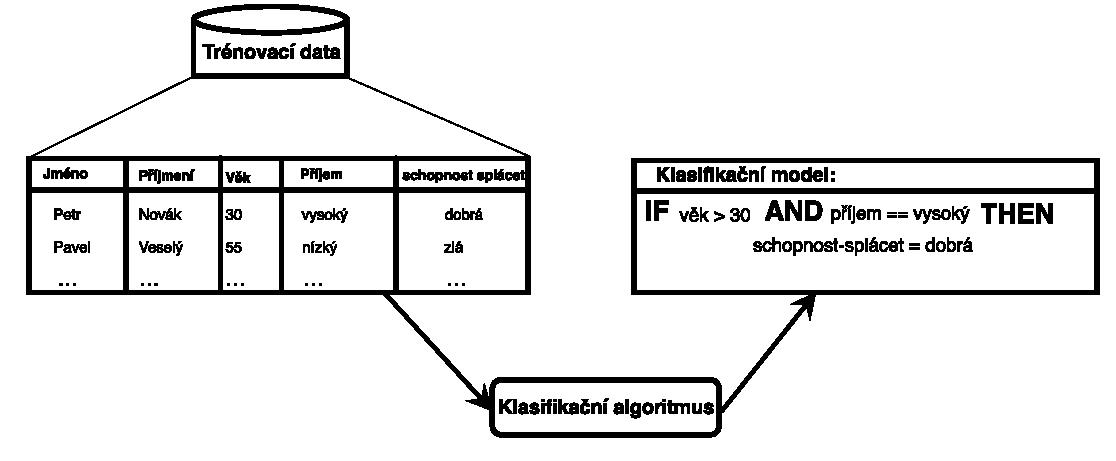
\includegraphics[width=\linewidth,height=2.0in]{obrazky/trenovacifaze.pdf}\\[1pt]
  \caption{Fáze trénování/učení klasifikačního modelu}
  \label{faze-trenovani}
\end{figure*}

Klasifikační model může mít různou podobu, například klasifikačních pravidel ve tvaru podmínek, rozhodovacího stromu, matematické formule nebo neuronové sítě. \cite{Han} Možné struktury těchto modelů je na obrázku \ref{modely-clf}.

\begin{figure*}[h]\centering
  \centering
  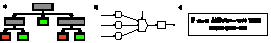
\includegraphics[width=\linewidth,height=1.5in]{obrazky/clf-modely.pdf}\\[1pt]
  \caption{Možné reprezentace klasifikačních modelu}
  \label{modely-clf}
\end{figure*}

V druhé fázi probíhá testování a vyhodnocení klasifikačního modelu, jinak řečeno určuje se míra úspěšnosti/neúspěšnosti klasifikace. Zde se pracuje s takzvanou validační množinou objektů. Třídy objektu této množiny jsou známe a díky tomu existuje vědomost a dokáže se určit míra úspěšnosti/neúspěšnosti na základě porovnání referenčních tříd s výsledky klasifikátora.\cite{Han}

Na základě výsledků z předešlého kroků je potřeba vykonat rozhodnutí zda model použít, anebo ne. Jestliže je model dostatečně přesný, je možné klasifikovat reálná data s neznámými třídami, jinak je potřeba model upravit nebo dokonce vytvořit nový. To vše je shrnuto na obrázku \ref{faze-testovani}.

\begin{figure*}[h]\centering
  \centering
  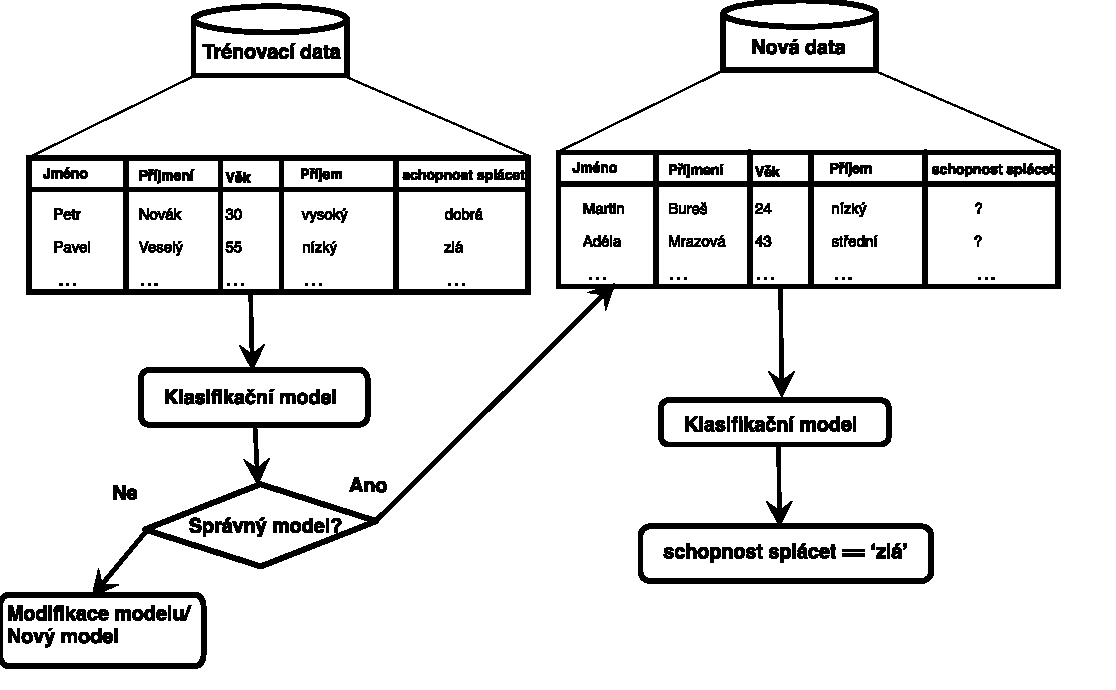
\includegraphics[width=\linewidth,height=2.7in]{obrazky/testovaci_faze.pdf}\\[1pt]
  \caption{Fáze testování klasifikačního modelu}
  \label{faze-testovani}
\end{figure*}

\subsection*{Shluková analýza}
Cílem tohoto dalšího typu dolovacích úloh je seskupování objektu do skupin na základě předem definovaných kritérií. Výsledkem této analýzy jsou homogenní skupiny. Objekty jedné skupiny by si měly být, co nejvíc podobné mezi sebou a zároveň, co nejméně podobné s ostatnímy objekty z jiných skupin. \cite{Mesakar}

Na obrázku \ref{cluster} jsou zákaznici  obchodu s elektronikou shlukování na základě utracených peněz a množství koupené elektroniky za jeden konkrétní měsíc.

\begin{figure*}[h]\centering
  \centering
  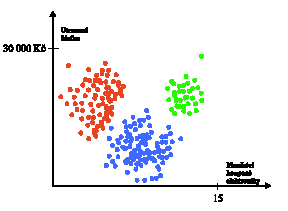
\includegraphics[width=4.0in,height=2.2in]{obrazky/slukovani_pr.pdf}\\[1pt]
  \caption{Shlukování zákazníků obchodu s elektronikou}
  \label{cluster}
\end{figure*}

\subsection*{Ostatní typy dolovacích úloh}
Zde si uvedeme dolovací úlohy, které nejsou v praxi tak časté jako výše zmíněné doposud, ale je vhodné se o nich zmínit.

\textbf{Analýza odlehlých objektů} patří do tohoto typu úloh a zajímá nás zde při tvorbě modelu hodnoty, které se liší od ostatních obvyklých hodnot \cite{Han}. Tato analýza může například odhalit podvodné použití kreditních karet. Když detekuje, že zákazník najednou provádí extrémně velké nákupy z daného účtu ve srovnání s běžně se vyskytujícími nákupy z tohoto účtu. 

Posledním typem dolovací úlohy, který tu bude zmíněn je \textbf{analýza evoluce}. Zde je cílem popisovat a modelovat pravidelnosti a trendy u objektů, jejichž chování se mění v čase \cite{Dunham}. Příkladem použití takové úlohy je pro analýzu podobnosti nebo vyhledávání periodicity. Výsledný model by mohl být použít pro předvídání budoucnosti a podpoře rozhodování.

\chapter{Metody dolování dat}
\label{metody}
Na výběr je z mnoha druhů algoritmů, které lze použít na získání znalostí z dat. Pro výběr správného algoritmu je potřeba si uvědomit, na jaké otázky by měl získat odpověď. 

Tato kapitola slouží k představení konkrétní metody pro úlohu dolování asociačných pravidel, klasifikace a shlukovou analýzu. První podkapitola se věnovuje popisu metod dolování asociačních pravidel, konkrétně algoritmů Apriori, metody FP stromu a Eclat. Dále následuje podkapitola zaměřená na metody klasifikace a to rozhodovací stromy, bayesovskou klasifikaci, neuronové sítě a $k$–nejbližších sousedů. A poslední podkapitola je věnovaná popisu metod shlukování, konkrétně shlukování založené na rozdělování, hierarchické shlukování a shlukování založené na hustotě.

\section{Metody pro asociační pravidla}
V této podkapitole jsou popsány a porovnány jednotlivé metody dolování asociačných pravidel. Prvně se představí algoritmus Apriori, potom metoda FP stromu a zakončí se stručním popisem algoritmu Eclat.

\subsection*{Algoritmus Apriori}
Tento velice znamý algoritmus slouží k získávání frekventovaných množín. Jeho princip je postavený na výuživání předešle znalosti o dříve získaných frekventovaných množinách, a proto má takový název. Když pokažde iteruje, aby generoval $(k+1)$-množinu ze získané frekvetované $k$-množiny, tak prochází databází. Dále má k dispozici Apriori vlastnost, která říká, že každa podmožina frekventované množiny, je taký frekventováná, tím taky dosahuje výšší eketivity. Proces, který využivá tuto vlastnost se skládá ze dvou kroků \cite{Han}:

\begin{enumerate}
    \item \textbf{Spojovací krok} -- K vytvoření $L_k$ (všech frekventovaných $k$-množin) je potřeba vygenerovat množinu kandidátů $C_k$ spojením množín z $L_{k-1}$. Nechť $l_1$ a $l_2$ jsou množiny $L_{k-1}$. Algoritmus předpokládá, že položky v množině jsou lexikografický seřazeny. Ke spojení dvou $(k-1)$-množin dojde, pokud jejich prvních $k-2$ prvků je shodných. Výsledná množina po spojení bude bude mít prvky $l_1[1]$, $l_1[2]$, ..., $l_1[k-1]$, $l_2[k-1]$ a přitom musí platit, že $l_1[k-1] < l_2[k-1]$. Tato podmínka zajišťuje, že se  v $L_k$ negenerují duplicity.
    \item \textbf{Vylučovací krok} -- množina $C_k$ je nadmnožinou $L_k$. Znamená to, že jí prvky mohou, ale taky nemusí být frekventovanými množinami. Pro zjištění výskytu každého kandidáta se provádí průchod databázi a to při velkém počtu položek je velmi neefektivní. Jako řešení se využívá Apriori vlastnost. Jestliže existuje $(k-1)$-množina, která je podmnožinou kandidátní $k$-množiny a není obsazená v $L_{k-1}$ (není frekventovaná), tak je daná kandidátní množina odstraněná.
\end{enumerate}

Pokud množina splňuje požadavek na minimální podporu, tak to splňují i všechny její podmnožiny. Tato vlastnost říká, že frekventované množiny jsou \textit{dole uzavřené} \cite{Dunham}.

Základní algoritmus Apriori je možno mnoha způsoby modifikovat, aby se docílilo jeho zlepšení. Příkladem takové modifikace může být zavedení hašování, přísnější redukce kandidátů nebo vzorkování. Tento algoritmus dokáže pracovat s transakční i relační databází. \cite{Han}
Na obrázku \ref{apriori} je ukázka, jak funguje algoritmus nad transakční databází.

\begin{figure*}[h]\centering
  \centering
  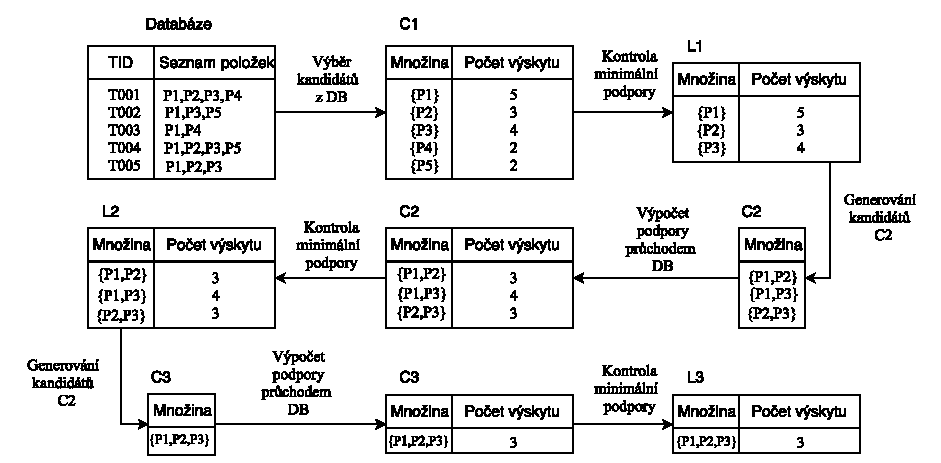
\includegraphics[width=\linewidth,height=2.7in]{obrazky/apriori_alg.pdf}\\[1pt]
  \caption{Algoritmus Apriori}
  \label{apriori}
\end{figure*}

\subsection*{Další metody}
Problémem u algoritmu Apriori se často stává generování kandidátů, kterých u větších databází může být velmi mnoho. Dalším problémem je potřeba neustále procházet databázi.

Vyřešením těchto problémů je zavedení metody vzrůstu frekventovaných množin. V první fázi této metody se provádí komprese databáze reprezentující frekventované položky do struktury nazvané \textbf{FP-strom} (strom frekventovaných množin). Tento strom se pak rozdělí do podmíněných FP-stromů, které jsou vytvořeny pro každou frekventovánou položku. Z těchto stromů jsou získány frekventované množiny. \cite{Han}

Dále existuje algoritmus \textbf{Eclat}, který je rekurzivní a funguje na principu prohledávání do hloubky v grafů oproti algoritmu Apriori, který je založen na principu prohledávání do šířky. Hlavní myšlenkou je rekurzivní práce s množinou identifikátorů položek. Při každém rekurzivním  voláním se pro každou množinu identifikátorů (kandidátů) ověřuje minimální podpora a následně jsou množiny navzájem kombinovaný. Tento proces pokračuje dokud existují množiny, které lze kombinovat. Eclat je řádově rychlejší a paměťové méně náročný než Apriori, ale nese stejné nevýhody jako generování kandidátů a průchod databází. \cite{Heaton}

\section{Metody pro klasifikace}
Existuje několik metod, které lze využít při řešení klasifikačních úloh. V této podkapitole se představí jednotlivé metody a porovnání mezi sebou.  Běžná kritéria pro porovnání klasifikačních metod jsou následující \cite{Han}:


\begin{itemize}
    \item \textbf{Přesnost} - udává kolikrát správně model vybral třídu na nových neznámých vzorcích,
    \item \textbf{Rychlost} - výpočetní složitost pro vygenerování a používání klasifikačního modelu,
    \item \textbf{Robustnost} - schopnost vytvořit správný model i z neuplných údajů,
    \item \textbf{Stabilita} - schopnost vytvořit správný model pro velké množství dat,
    \item \textbf{Interpretovatelnost} - složitost daného modelu pro pochopení.
\end{itemize}

\subsection*{Klasifikace pomocí rozhodovacích stromů}
Rozhodovací stromy patří mezi populární metody pro klasifikaci v oblasti dolovaní dat a to kvůli svým nepochybným kvalitám. Jak už z nazvu vyplivá, model je reprezentován grafem stromové struktury. Každý vnitřní uzel je označen jako rozhodovací, protože reprezentují test hodnoty jistého atributu, tím každý výsledek tvoří jednu větev stromu. Koncové uzly (listy) reprezentují třídu, do které je daný objekt klasifikován. \cite{Lior} Takový strom je uveden na obrázku \ref{strom_df}.

\begin{figure*}[h]\centering
  \centering
  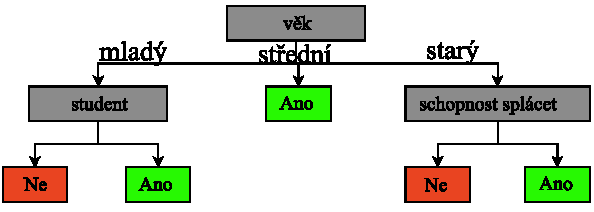
\includegraphics[width=5in,height=1.7in]{obrazky/rozhodovaci-strom.pdf}\\[1pt]
  \caption{Rozhodovací strom (převzaté z \cite{Han})}
  \label{strom_df}
\end{figure*}

Algoritmus pro vytvoření stromu je jednoduchý, ale celková problematika okolo klasifikace pomocí rozhodovacích stromu je rozsáhla a komplikovaná.

Velmi důležitým rozhodnutím při tvorbě stromu je, v jakém pořadí se dotazovat na hodnoty jednotlivých atributů. Řešením tohoto problému je speciální algoritmus, který funguje se seznamem atributů. Při každém kroku, kdy dochází k nárůstu stromu, se pro určitý atribut počítá \textbf{informační zisk}, který říká jak tento atribut dobře rozděluje data vzhledem na jejich cílovou třídu. Informační zisk závisí na hodnotě entropie. \textbf{Entropie} je míra (ne)určitosti informace. Po dokončeni vypočtu entropie a informačního zisku může se určit, který atribut má největší rozhodovací schopnost a bude použít při tvorbě stromu jako aktuální. \cite{Dunham}

Dalším problémem při vytvářeni takového stromu i vlivem datového šumu je vznik větvi, které dělají strom mnohem složitější, ale i méně kvalitním z hlediska předpovědi.  Tim vzniká potřeba, aby se tyto větve odstranily. Základní metody na odstranění těchto větví jsou následující \cite{Han}:

\begin{itemize}
    \item \textbf{Prepruning} – odstranění přebytečných větev probíhá při tvorbě stromu. Tato metoda je rychlejší.
    \item \textbf{Postpruning} - odstranění přebytečných větev probíhá až po jeho úplném vytvoření. Tato metoda je spolehlivější.
\end{itemize}


Mezi další výzvy, které je potřeba řešit při tvorbě rozhodovacích stromu, patří určovaní hloubky, do které může strom růst, zpracovaní spojitých atributu,  zpracovaní atributu s jiným ohodnocením nebo zvýšeni efektivity vypočtu. Existuje mnoho složitějších metod postavených na základě rozhodovacího stromu. Jedna z takových metod je \textbf{náhodný les}. Tato metoda vytváří více stromu a při samotné klasifikaci je výsledkem nejčastější hodnota tříd získaná jednotlivými stromy  \cite{Han}.

Mezi výhody rozhodovacích stromů patří jednoduchý převod na klasifikační pravidla, nízká náročnost na množství výpočtů při klasifikaci, schopnost pracovat se spojitými i diskrétními hodnotami a jasná indikace nejdůležitějších atributů pro predikci. Jako nevýhody lze uvést vetší sklon k chybám v případě klasifikace do většího množství tříd nebo potenciální časová náročnost k vytvoření stromu. \cite{Lior}

\subsection*{Bayesovká klasifikace}
Tato klasifikační metoda provádí klasifikaci na principu založeny na statistice a pravděpodobnosti. Myšlenka této metody je, že pomocí statistických metod určí s jakou  pravděpodobnosti nový vzorek patří do jednotlivých tříd. Vzorek následně bude zaražen do třídy, pro kterou má vypočítanou nejvyšší pravděpodobnost. 

Pro porozumění jednoduché bayesovké klasifikaci je zavedeno následující pojmy \cite{Han}:

\begin{itemize}
    \item $S$ - množina všech vzorků (trénovacích dat)
    \item $C_1, C_2,...,C_m$ - jednotlivé třídy, do kterých jsou vzorky z množiny $S$ klasifikované. Symbol $m$ udává celkový počet těchto tříd.
    \item $s_i$ - počet prvků z množiny $S$, které jsou klasifikované do třídy $C_i$, kde $i=1,...,m$
    \item $A_1, A_2,...,A_n$ - jednotlivé atributy, pomocí kterých se bude klasifikovat
    \item $X = (x_1,X_2,...,x_n)$, kde $x_i$ je hodnota atributu $A_i$ pro všechna $i=1,...,m$, značí testovací vzorek, který má být klasifikován do nějaké třídy.
    \item $P(C_i|X)$, kde $i=1,...,m$ udává podmíněnou pravděpodobnost toho, že libovolný vzorek padne do třídy $C_i$, pokud je známo, že vzorek má atributy shodné s prvkem $X$.
\end{itemize}

Úkol je tedy najít takové $i$, pro které je hodnota $P(C_i|X)$ největší, přičemž je vzorek $X$ pak zařazen do třídy $C_i$. Podle Bayesova vzorce \ref{bayes} platí:
\begin{equation}
	 P(C_i|X) =\frac{P(X|C_i)P(C_i)}{P(X)}
	\label{bayes}
\end{equation}
$P(X)$ je pro konkrétní vzorek $X$ konstantou, a tak stačí hledat třídu $C_i$, pro kterou je hodnota výrazu $P(X|C_i)P(C_i)$ maximální:
\begin{itemize}
    \item $P(C_i)$ je pravděpodobnost že libovolný zvolený prvek patří do třídy $C_i$, která se vypočítá pomocí vzorce \ref{bayes2}:
    
    \begin{equation}
	    P(C_i) =\frac{s_i}{|S|}
	    \label{bayes2}
    \end{equation}
kde $|S|$ značí počet prvků v této množině (kardinalitu).
    \item $P(X|C_i)$ je pravděpodobnost, že libovolný prvek vybraný ze třídy $C_i$ bude mít stejné hodnoty atributů jako prvek $X$, kterou získáme pomocí vzorce \ref{bayes3}:
    \begin{equation}
	    P(X|C_i) = \prod_{k=1}^n P(X_k|Ci)
	    \label{bayes3}
    \end{equation}
\end{itemize}

Tento typ klasifikace se dá aplikovat například při klasifikaci textu, filtrování spamu nebo kategorizace dokumentů. Mezi jeho silné stránky patří jeho jednoduchost a jeho efektivnost. Naopak jeho slabou stránkou je předpoklad, že atributy jsou nezávislými mezi sebou \cite{Rish}.

\subsection*{Klasifikace pomocí neuronových sítí}
Tato další klasifikační metoda je inspirovaná činností biologického neuronů. Obvykle se neuronová síť skládá z několika umělých neuronu. Umělý neuron je složen z těla (biologický označeno soma), vstupy (dendrity) a výstup (axon) \cite{Kantardzic}, který je možné vidět na obrázku \ref{neuron}.

\begin{figure*}[h]\centering
  \centering
  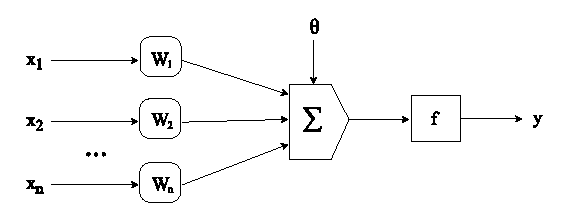
\includegraphics[width=\linewidth,height=2.2in]{obrazky/Umely-neuron.pdf}\\[1pt]
  \caption{Umělý neuron}
  \label{neuron}
\end{figure*}

Jeho činnost spočívá v zavedení na jeho vstup hodnoty $x_1,x_2,...x_n$, které jsou získané ze vstupních dat nebo z výstupu jiných neuronů. Dále vstupné hodnoty jsou násobené váhovými hodnotami $w_1,w_2,...,w_n$, které reprezentují synapse u biologického neuronu, aby přijatý signál zesílili nebo zeslabili. Z těchto hodnot je vypočítána suma podle vzorce \ref{neuron_eq}:

    \begin{equation}
	    \sum_{i=1}^n w_ix_i + \theta,
	    \label{neuron_eq}
    \end{equation}
kde $\theta$ je vnitřní konstanta daného neuronu označována jako bias a je k této sumě vždy přičtena. Dal se tato suma přivede  na vstup aktivační funkce, která může generovat skokový nebo spojitý výstup $y$. Tento výstup může být buď vstupem dalších neuronů nebo může tvořit výstupní hodnotu, na základě které bude provedena klasifikace konkrétního vzorku. Tato uvedena činnost platí pro každý neuron, který se nachází v síti. \cite{Han}

Počet neuronů a jejich vzájemné propojení v síti určuje takzvaná architektura (topologie) neuronové sítě. Existuje mnoho odlišných architektur, ale nejběžnější způsob je rozdělit síť do několika vrstev. Typ neuronu je určen konkrétní vrstvou. V zásadě můžeme rozlišovat dva hlavní typy architektur neuronových síti \cite{Dunham}:

\begin{enumerate}
    \item \textbf{Dopředná síť} - neurony lze vždy rozdělit do vrstev, které jsou uspořádány tak, že spoje mezi neurony vedou jen z jedné vrstvy do další vrstvy, takže se informace zpracovává jedním směrem od vstupu k výstupu. Tento typ se využívá v případě, kdy je známá kompletní vstupní informace.
    \item \textbf{Rekurentní síť } - zde dochází k vytvoření cyklu takový nejjednodušším příkladem je zpětná vazba neuronu, jehož výstup je zároveň jeho vstupem. Signál, který přišel vstupní vrstvou, cirkuluje do doby, než se stav v síti neustáli. Když je stav ustálen, tak je možné přečíst výstup. Nejčastěji se využívá, když pro výsledek je důležité časová posloupnost vstupních dat.
\end{enumerate}

Když se vybere architektura, typ učení a učící algoritmus, tak se vy tváří model neuronové sítě. Nejznámější modely neuronových sítí jsou sítě, které používají algoritmus \textbf{zpětného šíření} (v angličtině Backpropagation). 

Nejjednodušším modelem je \textbf{Perceptron}, který obsahuje jeden neuron s více vstupy a jeden výstup. Takový Perceptron se používá pro klasifikaci do dvou tříd. Dalšími modely jsou vícevrstvý Perceptron (v angličtině multilayer perceptron se zkratkou MLP), Kohonenovy mapy nebo RBF (Radial Basic Function) sítě. \cite{Dunham}

Neuronová síť se zpětným šířením používá architekturu dopřední sítě a funguje tím, že na začátku jsou váhy a biasy jednotlivých neuronů nastaveny na malá náhodná čísla. Na vstupní vrstvu je přiveden první vzorek z trénovací množiny. V případě učení s učitelem musí vzorek obsahovat i požadovaný výstup. Hodnoty ze vstupní vrstvy se šíří do první skryté vrstvy, kde se nové hodnoty šíří dál a to pokračuje až na výstupní vrstvu, která vygeneruje výstup. Vygenerovaný výstup se porovná s požadovaným výstupem a vypočítá se chyba. Tato chyba je z výstupu šířena celou sítí nazpět na vstup a přitom jednotlivé neurony mění hodnoty váh a biasu, tak aby byla chyba minimální. Tyto kroky probíhají pro každý vzorek z tréningové množiny. Jako výhodu tohoto algoritmu můžeme uvést jeho jednoduchost, univerzálnost a robustnost a jako nevýhodou je časová náročnost trénovacího procesů. \cite{Han}

Neuronové sítě dávají možnost pracovat na vstupu a výstupu s diskrétními a spojitými hodnotami. Oproti ostatním metodám jsou ve většině případů efektivnější. Jednu z největších nevýhod neuronových síti je obtížnost interpretovat jejích výsledky a taky to, že vstupné data by měly být omezena jen na intervalu 0 až 1. \cite{Kantardzic}

\subsection*{K – nejbližších sousedů}
Tato metoda pracuje na základě porovnávání podobnosti trénovacích a testovacích vzorků, kde konkrétní vzorek je reprezentován $n$ číselnými atributy se stejnou váhou. Jednotlivé vzorky lze chápat jako body v $n$-dimenzionálním prostoru. Když klasifikujeme neznámý prvek, tak se vybírá $k$ nejbližších vzorů z trénovacích dat a tento prvek je zařazen do třídy s největším zastoupením právě u těchto $k$ vybraných vzorů. Mezi dvěma prvky $X = (x_1,x_2,...,x_n)$ a $Y = (y_1,y_2,...,y_n)$ se nejbližší vzdálenost počítá pomocí tzv. Euklidovské vzdálenosti podle následujícího vzorce \ref{k_eq}. \cite{Han}

    \begin{equation}
	    d(X,Y)=\sqrt{\sum_{i=1}^n(x_i-y_i)^2}
	    \label{k_eq}
    \end{equation}

\subsection*{Další klasifikační metody}
Jedna z dalších metod klasifikace je pomocí \textbf{genetických algoritmu}, které jsou založené na principu přírodního vývoje a genetických vlastnostech. V přírodě rodiče nějakého živočišného tvorů mají jisté geny a tyto geny následně zdědí jejich potomek. Pokud tento potomek má být silný jedinec, tak si vezme od každého rodiče ten \uv{lepší} gen. Gen se v různých organismech zakódovává pomocí nějakého chemického vzorce. Tento nápad se uplatňuje i v genetických algoritmech, ale místo chemického vzorce se používá obyčejné řetězce. \cite{Han}

Další metoda klasifikace je založena na \textbf{fuzzy množinách}. Princip této metody je určování míru náležitosti atributu k jednotlivým třídám. Tím se diskrétní rozhodování stává jemnější pro specifikaci koeficientů z intervalu 0 až 1. \cite{Holecek}

\section{Metody pro shlukovou analýzu}

V této podkapitole se představí a porovná nejznámější metody pro shlukovou analýzu. Taková běžná kritéria na porovnání těchto metod jsou následující \cite{Han}:

\begin{itemize}
    \item způsobilost zpracovat rozsáhlé databáze
    \item způsobilost zpracovat různé typy atributů
    \item způsobilost vytvořit shluky různého tvaru
    \item způsobilost vyrovnat se s daty obsahující šum
    \item způsobilost zpracovat vysokodimenzionální data
\end{itemize}   

Shlukovací metody lze všeobecně rozdělit do několika skupin. Z metod založených na rozdělování se představí metoda k-means a k-medoids. Dále jsou popsané hierarchické metody a metody založené na rozdělování. Na závěr podkapitoly jsou stručně zmíněné další skupiny shlukovacích metod.

\subsection*{Metody založené na rozdělování}
Skupina těchto metod je založena na rozdělování $n$ vzorků do $k$ skupin a přitom musí platit, že $k \leq n$. Dále musí platit, že každá skupina musí obsahovat alespoň jeden vzorek. Princip algoritmu je v náhodném vybrání $k$ vzorků, které na počátku reprezentují jednotlivé shluky. Potom se iterativně hledají vzorky, které nejlépe vystihují daný shluk. Aby se dosahlo konečného výsledku, tak se vyživájí různé heuristiky, jakými jsou například k-means nebo k-medoids. \cite{Dunham}

Shlukování \textbf{k-means} je založeno na bázi nalezení středového bodu shluku.Vzorky jsou dále rozděleny a přiřazeny ke středovému bodu, který je k nim nejblíže. Když se používá shlukování tímto algoritmem je třeba uvědomění, že výsledky se mohou každým spouštěním lišit, neboť výběr středu shluků je prováděn náhodně. \cite{Kantardzic}

Shlukování \textbf{k-medoids} se velmi podobá shlukování k-means. Liší se zásadně v tom, že v algoritmu k-medoids není shluk reprezentován svým středem, ale vzorkem, který je nejblíže středu. Kvůli teto vlastnosti je algoritmus robustnější v případě přítomnosti odlehlých vzorků. \cite{Han}

Vhodné použití těchto metod je například pro hledání shluků, které mají kulatý tvar, z datasetu o velikosti menší až středně velký. Jako nevýhodou těchto metod je fakt, že je třeba předem určit počet shluků.

\subsection*{Hierarchické metody}
Tato metoda shlukování na základě předem definované metriky vypočítá vzdálenost mezi vzorky. Díky této vzdálenosti jsou vzorky hierarchicky rozdělené a tím vzniká strom shluků. Rozdělení je možné provést buď shora dolů nebo zdola nahoru, tzn. že vzorky se buď postupně rozdělují nebo spojují do shluků. Jako konkrétní příklad je možné uvést rozdělující metodu AGNES (AGglomerative NESting) a spojující metodu DIANA (Divisive ANAlysis). \cite{Han} 

Tyto metody jsou rychlejší než metody založené na rozdělování, ale jejich nevýhodou je menší přesnost, a že pokud některé shluky sloučíme nebo naopak rozdělíme, tak už není možné nikdy tyto shluky zpět rozdělit nebo spojit.

\subsection*{Metody založené na hustotě}
Tyto metody uvažují oblasti s velkou hustotou vzorků v prostoru dát za shluky, které jsou od sebe oddělené oblastmi s malou hustotou vyskytujících se vzorků. Příkladem takových metod jsou DBSCAN a DENCLUE. \cite{Han}

Metoda \textbf{DBSCAN} závisí na dvou klíčových parametrech, a to velikost okolí a minimální počet bodů. Jestliže je ve vzdálenosti okolí bodů $P$ víc bodů než stanovené minimum, tak se bod $P$ vyhlásí za tzv. jádro, to znamená, že bod $P$ spolu s body z jeho okolí tvoří jeden shluk. \cite{Kantardzic}

Metoda \textbf{DENCLUE} využívá distribuční funkce hustot. Každý konkrétní vzorek je možné modelovat pomocí funkce vlivu v jeho okolí. Součtem jednotlivých funkcí všech bodů (vzorků) v prostoru dát vytvoříme celkovou funkci hustoty datového prostoru. Shluky jsou vytvořené díky místům prostoru, kde se nachází lokální maxima celkové funkce hustoty. \cite{Han}

Výhodou těchto metod je, že dokážou nacházet shluky různých tvarů a jsou schopné zároveň se vypořádat s výskytem šumu a odlehlých hodnot v datech. 

\subsection*{Další shlukovací metody}
Příkladem dalších metod slukování je \textbf{metoda založená na modelech}, jejímž cílem je najít specifický model, který co nejpřesněji odpovídá zdrojovým datům. Na základě optimálního modelu se vytvářejí shluky. Základní myšlenkou \textbf{metody založené na mřížce} je rozdělit prostor vzorků do buněk ve tvaru mřížky, a následně všechny operace shlukování se provádí nad touto mřížkou, a to dělá tyto metody rychlejšími. \textbf{Metody pro shlukování vysoce-dimensionálních dat} jsou navrženy, aby odstranili nedokonalosti většiny typů shlukování, a to neschopnost práce s větším počtem atributů. \cite{Han}

\chapter{Jazyk Python a dostupné knihovny pro dolování dat}
\label{python}
Předtím než se začne řešit dolovácí úloha, je potřeba se rozhodnout jaký nástroj se k tomu vybere. Tyto nástroje by měli usnadnit už tak komplikovaný proces dolování dat. K dispozici jsou komerční, ale i volně dostupné nástroje. 

Tyto volně dostupné nástroje se už vyvíjí přes 20 let. Jejich cíl je nabídnout všem odborníkům na tuto oblast zajímavou alternativu ke komerčním nástrojům. Častokrát jsou k dispozici ve formě integrovaných prostředí nebo specializovaných balíčků nad rámec standardních programovacích jazyků, které jsou často open source (zdrojové kódy jsou volně dostupné a zdarma). Příkladem takových nástrojů může být RapidMiner, Orange, Weka, KNIME, programovací jazyk R a Python.  \cite{Jovic1}

První část kapitoly je zaměřená na stručný popis jazyka Python a jeho dostupných knihoven, které dohromady tvoří jeden z nejoblíbenějších nástrojů pro datovou analýzu. Druhá část kapitoly je zaměřená na popis podpory konkrétních knihoven jazyka Python v oblasti dolování dat.

\section{Jazyk Python a jeho knihovny}
\label{knihovny}
V roce 1991 se objevil tento vysokoúrovňový interpretovaný skriptovací jazyk, který navrhl Guido van Rossum. Díky své jednoduchostí, přehledné syntaxi, čitelnosti, multiplatformnosti a obrovské možnosti použitelnosti se teď tento jazyk těší velké popularitě \cite{Stancin}. S porovnáním s ostatnímá programovacímá jazykama používá pro bloky kódu odsazení pomocí mezera místo složených závorek. Nabízí podporu pro objektově orientované programování, funkcionální a imperativní.

Do jádra jazyka Python nebylo integrováno mnoho nástrojů pro analýzu a modelování dat. Tento nedostatek byl zaplněn vytvořením velkého množství knihoven. Jednotlivé knihovny jsou zaměřené na rozdílné části dolování a proto se kombinují dohromady a společně tvoří vykonné, lehce použitelné prostředí pro dolování dat. Dále budou stručně popsané knihovny, které se využili v experimentální části této práce.

\subsection*{Jupyter Notebook}
Tento balíček jazyka Python nabízí interaktivní grafické prostředí v prohlížeči, kde je možné spouštět programy vytvořené v nejrůznějších jazycích \cite{jupyter}. Má formu webové aplikace, která slouží pro vytváření oddělených bloků kódu, které je možné spouštět samostatně a zároveň tyto bloky můžou tvořit celistvý program. Zároveň kromě bloku kódu nabízí možnost přidat vizualizaci nebo vysvětlující text v různých formátech.

\subsection*{NumPy}
Je to základní knihovna jazyka Python, která byla speciálně vytvořená pro vědecké výpočty \cite{numpy}. Tato knihovna disponuje vysoce výkoným multidimenzionálním polem označené \verb|ndarray|, kde všechny prvky musí být stejného datového typu. Nad tímto polem jsou k dispozici různé funkce jako například přístup k jednotlivým dimenzím pole nebo jejich transformace. Dále tato knihovna obsahuje rozhraní pro matematické, agregační a porovnávací operace. 

\subsection*{Pandas}
Tato knihovna, která je postavená na knihovně NumPy, je velice významná, protože umožňuje manipulaci a analýzu velkého množství dat \cite{pandas}. Tato knihovna má základní prvek, který je jednodimenzionálním polem typu \verb|ndarray| (z NumPy) a je označeno jako \verb|Series|. Na tomto prvků je postaven další významný prvek knihovny, který se nazývá \verb|DataFrame|. Tento prvek má podobu dvou dimenzionální tabulkové struktury, která může obsahovat různé typy dat (numerická i textová). Rozhraní toho prvků nabízí snadnou manipulaci s daty jako například čtení, aktualizace, přidávání, odstraňování, a to buď podle názvu sloupců nebo indexů řádků. V případě, že data obsahují chybějící hodnoty, tak jsou k dispozici funkce, které odstraní nebo nahradí tyto hodnoty. Důležitou součastí \verb|DataFrame| jsou sumarizující funkce, které zobrazují přehledné charakteristiku uložených dat. Pomocí této knihovně je možné číst data z různých souborů (csv, xls, atd.) nebo databází, a také do nich zapisovat.

\subsection*{Matplotlib}
Jedná se o oblíbenou knihovnu jazyka Python pro vizualizaci dat \cite{matplotlib}. Tato knihovna je skvělým doplňkem ke knihovně NumPy. Je možné zde tvořit různé typy grafu jako jednoduché klasické grafy funkci o jedné proměnné, polární grafy, koláčové grafy, histogramy apod. Umožňuje uživatelům mít plnou kontrolu nad vlastnostmi písmen, čar, barev, stylů a os stejně jako například v MATLABu\footnote{Komerční nástroj pro vědecké a technické výpočty, analýzu dat, vizualizaci a vývoj algoritmů}. Také poskytuje kompatibilitu s různými knihovnami a balíčky třetích stran, které rozšiřují jeho funkčnost například knihovna seaborn.

\subsection*{Scikit-learn}
Je to knihovna pro analýzu dat a z nich získávání znalostí pomocí algoritmu strojového učení \cite{scikit-learn} z roku 2007, která byla naprogramována hlavně v jazyce Python, ale obsahuje kód i v jiných jazycích (C a C++). Je založená na výše uvedených knihovnách. Nabízí různé algoritmy strojového učení jak s učitelem, tak bez učitele. Hlavně se jedná o třídy algoritmu pro klasifikaci, regresi nebo shlukování. 

Tato knihovna se považuje za takový standard v oblasti strojového učení nebo dolování dat v prostředí jazyka Python. Pokud někdo, kdo právě začíná s dolováním dat a chce k tomu použít jazyk Python, tak se mu doporučí použít knihovnu scikit-learn. 

\subsection*{Mlxtend}
Toto je další knihovna, která nabízí algoritmy pro strojové učení a dolování dát \cite{mlxtend}. Mlxtend je napsáná v jazyce Python a byla vytvořená v roce 2014. Obsahuje jednoduché rozhraní, které je kompatibilní s dalšíma knihovnama strojového učení jako například scikit-learn. K dispozici jsou primárně algoritmy ze tříd klasifikace, regresi nebo dolování frekventovaných množín.
\subsection*{PyCaret}
Je to nejmladší alternativa ke knihovnám scikit-learn a mlxtend. Je napsaná v jazyce Python a byla vytvořená v roce 2020. Jedná se o knihovnu pro strojové učení, která dokáže nahradit spousta řádků kódu jen pár příkazy, tím že automatizuje pracovní postupy strojového učení \cite{PyCaret}. Nabízí algoritmy ze tříd pro klasifikaci, vytvoření asociačních pravidel, regresi a shlukování.

\section{Dolování dat v dostupných knihovnách}
\label{knihovny_2}
Úkolem této podkapitoly je zaměřit se na knihovny scikit-learn, mlxtend a PyCaret a představit jejích možnosti použití v procesu dolování dat. Postupně jsou ukázané funkce a moduly jednotlivých knihoven, které pokrývají algoritmy představené v předchozí kapitole \ref{metody}. Jejích implementace je demonstrována v následující kapitole \ref{experimenty}.

\subsection{Scikit-learn}
\subsubsection*{Asociační pravidla}
Knihovna scikit-learn nabízí velké množství algoritmů pro učení s učitelem nebo bez učitele, takže algoritmy hlavně řeší úlohy pro klasifikaci, regresi a shlukování. V této knihovně neexistuje žádný modul, třída a ani funkce, která by nabízela algoritmy pro asociační pravidla \cite{Stancin}. 
\subsubsection*{Klasifikace}
Klasifikační algoritmy a modely jsou nabízené touto knihovnou formou objektů, který musí mít následující dvě důležité funkce: \verb|fit()| a \verb|predict()|. Tento objekt se nazývá \verb|estimator|.

Modul \verb|sklearn.tree| nabízí podporu pro tvorbu klasifikačního modelu ve formě \textbf{rozhodovacího stromů}. Tvorba takového modelu je realizována pomocí třídy \begin{verbatim}DecisionTreeClassifier(),\end{verbatim} která na vstupu přijímá velké množství parametrů pro možnost úpravy procesu tvorby tohoto modelu. Po vytvoření modelu je možné tento model pomocí funkce \verb|fit()| trénovat na trénovacích datech a následně klasifikovat třídy pro neznáme objekty pomocí funkce \verb|predict()|. 

Model \textbf{náhodného lesa} se vytvoří pomocí třídy \verb|RandomForestClassifier()| nabízen modulem \verb|sklearn.ensemble|. Při tvorbě tohoto modelu se vytvoří určitý počet rozhodovacích stromu. Tento počet se nastaví pomocí parametru třídy.

\textbf{Bayesovká klasifikace} nabízená modulem \verb|sklearn.naive_bayes|. Existují různé třídy pro různé algoritmy Bayesovské klasifikace například \verb|GaussianNB()| implementuje algoritmus, který počítá s tím, že vzorky jednotlivých tříd mají Gaussovo rozdělení. Pro kategorická data existuje třída \verb|CategoricalNB()|.

Modul \verb|sklearn.neural_network| nabízí modely na bázi \textbf{neuronových sítí}. Takový klasifikačním model jde vytvořit pomocí třídy \verb|MLPClassifier()|. Tato třída nabízí spousta parametrů, které mohou upravit proces tvorby tohoto modelu.

Klasifikační model pomocí algoritmu \textbf{k-nejbližších sousedů} je implementovan třídou \verb|KNeighborsClassifier()| z modulu \verb|sklearn.neighbors|.

\subsubsection*{Shluková analýza}
Všechny populární algoritmy pro shlukovou analýzu se nachází v modulu \verb|sklearn.cluster|.
Shlukováním založené na rozdělování má zástupce formou \textbf{k-means}, který se vytvoří pomocí třídy \verb|KMeans()|. Vykonání algoritmu a zařazení dat do shluků probíhá pomoci funkce \verb|fit_predict()|.

Hierarchické shlukování se vytvoří pomocí třídy \verb|AgglomerativeClustering()|, který přijímá jako parametr buď počet shluků, do které má zařadit data nebo práh vzdálenosti, při které se shluky nad touto vzdálenosti mezi sebou nebudu spojovat. 

Tento modul poskytuje podporu i pro shlukování založené na hustotě. Konkrétně v podobě algoritmu DBSCAN, který je reprezentován třídou \verb|DBSCAN()|, který přijímá povinně dva parametry: vzdálenost okolí bodů a minimální počet bodů, které se nachází v okolí.

\subsection{Mlxtend}
\subsubsection*{Asociační pravidla}
Knihovna nabízí modul \verb|mlxtend.frequent_patterns| pro tvoření frekventovaných množín a z nich asociační pravidla. Tento modul obsahuje dva algoritmy pro dolování frekventovaných množin. Prvním algoritmem je algoritmus \textbf{Apriori}, který je implementován pomocí funkce \verb|apriori()|. Druhým algoritmem je metoda \textbf{FP-stromu}, který je implementován pomocí funkce \verb|fpgrowth()|. 

Poté co se vytvoří frekventovaná množina ze vstupních dat, tak se zavolá funkce \begin{verbatim}
    association_rules(),
\end{verbatim}která generuje asociační pravidla.

\subsubsection*{Klasifikace}
Pro klasifikační algoritmy tato knihovna nabízí modul \verb|mlxtend.classifier|. Z klasifikačných metod představených v předchozí kapitole \ref{metody} mlxtend nabízí jen klasifikaci pomocí \textbf{neuronových sítí}, ale zato několik různých variant. 

Třída \verb|Perceptron()| implementuje model, který obsahuje jediný umělý neuron. Tento model se hodí na binární klasifikaci (klasifikuje se do dvou tříd). 

Další třída, která implementuje model pro takový typ klasifikačních úloh, je \verb|Adaline()|, který vychází z anglického spojení slov \textit{ADAptive LInear NEuron}. Rozdíl oproti klasického Perceptronu je ve fázi učení, kde váhy jsou upravené podle váženého součtu vstupů.

Poslední třídá \verb|MultiLayerPerceptron()| implementuje model vícevrstvého Perceptronu podobný tomu z knihovny \textit{scikit-learn}.

\subsubsection*{Shluková analýza}
Pro shlukování je k dispozici modul \verb|mlxtend.cluster|, který nabízí jediný algoritmus pro shlukování a to \textbf{k-means} implementován pomocí funkce \verb|Kmeans()|.

\subsection{PyCaret}
\subsubsection*{Asociační pravidla}
PyCaret pro asociační pravidla má k dispozici modul \verb|pycaret.arules|.  Zde jde implementován algoritmus \textbf{Apriori} pomocí funkce \verb|create_model()|, která zároveň generuje asociační pravidla. Funkce přijímá argumenty, které určují například minimální podporu a spolehlivost. 

\subsubsection*{Klasifikace}
Klasifikaci zde zajišťuje modul \verb|pycaret.classification|. Pomocí funkce \verb|models()| se zobrazí všechny dostupné algoritmy pro klasifikaci. Dále je možné použít funkci \begin{verbatim}
    compare_models(),
\end{verbatim}která implementované algoritmy porovnává a ukazuje, který model je nejvhodnější pro vybranou datovou sadu. Poté se použije funkce \verb|create_model()|, která vytvoří daný nejvhodnější model. Pokud je potřeba vytvořit jiný model například rozhodovací stromy, tak se to určí argumentem pro tuto funkci: \verb|create_model('dt')|. 

Jsou zde k dispozici všechny prezentované klasifikační algoritmy stejně jako v knihovně \textit{scikit-learn}.

\subsubsection*{Shluková analýza}
Pro shlukování PyCaret nabízí modul \verb|pycaret.clustering|. Jsou zde k dispozici stejné funkce jako u klasifikace prezentované výše, takže následuje stejný postup. 

Například když se má vytvořit model podle metody založené na rozdělování pomocí algoritmu k-means, tak se to realizuje následujícím způsobem: \verb|create_model('kmeans')|.

\chapter{Experimenty v dostupných knihovnách jazyka Python}
\label{experimenty}
Tato kapitola se zaměřuje na popis experimentů, které byly vyhotovené pro demonstraci možnosti jednotlivých knihoven pro dolování dat jazyka Python. 

Celkové půjde o tři experimenty. Každý experiment se bude zaměřovat na jeden typ dolovácí úlohy. Konkrétně se bude jednat o dolování asociačních pravidel, klasifikaci a shlukovou analýzu.

Každý experiment má jasně definovanou strukturu, která se skládá z představení experimentu, popis a ukázky datové sady, implementace experimentu pomocí knihoven scikit-learn, mlxtedn a PyCaret, a nakonec následuje shrnutí experimentu. Obecná teorie k daným dolovacím úlohám se nachází v podkapitole \ref{typyuloh} a popis jednotlivých metod a algoritmů jsou v kapitole \ref{metody}. Bylo použito prostředí \textit{Jupyter Notebooku}, které bylo představeno v podkapitole \ref{knihovny}, pro realizaci jednotlivých experimentů. 

\section{Asociační pravidla}
\label{asociacni-pravidla}
Tento první experiment prezentuje příklad dolování asociačních pravidel. Experiment je realizován nad datovou sadou pekárny z Edinburghu. Cílem tohoto experimentu je provést analýzu nákupního košíku této pekárny.  Jinak řečeno zjistit, které produkty se často prodávají dohromady a tím pomoct pekárny, aby např. navrhla nějakou akci v budoucnu pro tyto produkty, nebo které produkty by měla doporučit při koupi nějakého jiného produktu. 

Dále nás bude zajímat, jak jednotlivé knihovny zvládnou tento úkol pomocí algoritmů, které nabízí a byly představeny v podkapitole \ref{knihovny_2}.

\subsection*{Datová sada pekárny z Edinburghu}
Tato datová sada, která je dostupná online\footnote{\url{https://www.kaggle.com/datasets/mittalvasu95/the-bread-basket?resource=download}}, obsahuje 20 507 záznamu, kde každý záznam prezentuje konkrétní prodej položky, která tato pekárna prodala online v období mezi říjen roku 2016 až  do dubna roku 2017. Každý záznam je popsán 5 atributy. Konkrétně se jedná o číslo transakce, položka, datum, období během dne a období v týdnu. Číslo transakce popisuje zda prodaná položka byla součástí většího nákupu. Položká popisuje konkrétní produkt například chleb. Období během dne udává zda prodej byl ráno nebo odpoledne a období v týdnu popisuje zda prodej byl vykonán v pracovních dnech nebo o víkendu.

Datová sada se nachází v textovém souboru typu csv (zkratka z angličtiny comma-separated values). Tento soubor obsahuje textové hodnoty, které jsou rozdělené znakem středník. 

Pomocí funkce z knihovny \textit{pandas} představené v podkapitole \ref{knihovny} načteme datovou sadu a vytvoříme z ní \verb|DataFrame|. Tento krok je zobrazen v následující ukázce:

\begin{mdframed}
\begin{lstlisting}[language=Python]
#nacteni knivony
import pandas as pd

#nacteni dat z csv souboru
df = pd.read_csv("datasets/bread-basket.csv")

\end{lstlisting}   
\end{mdframed}

Dále knihovna \textit{pandas} nabízí několik funkcí, které slouží k prozkoumání datové sady. Například funkce \verb|info()| zobrazí datové typy jednotlivých atributů. Pomocí funkce \verb|isna()| bylo zjištěno, že datová sada neobsahuje žádné chybějící hodnoty. 

Pomocí knihoven \textit{matplotlib} a \textit{seaborn} se zobrazí 10 nejprodávanějších položek pekárny, které je možné vidět na obrázku \ref{top10}. 

\begin{figure*}[h]\centering
  \centering
  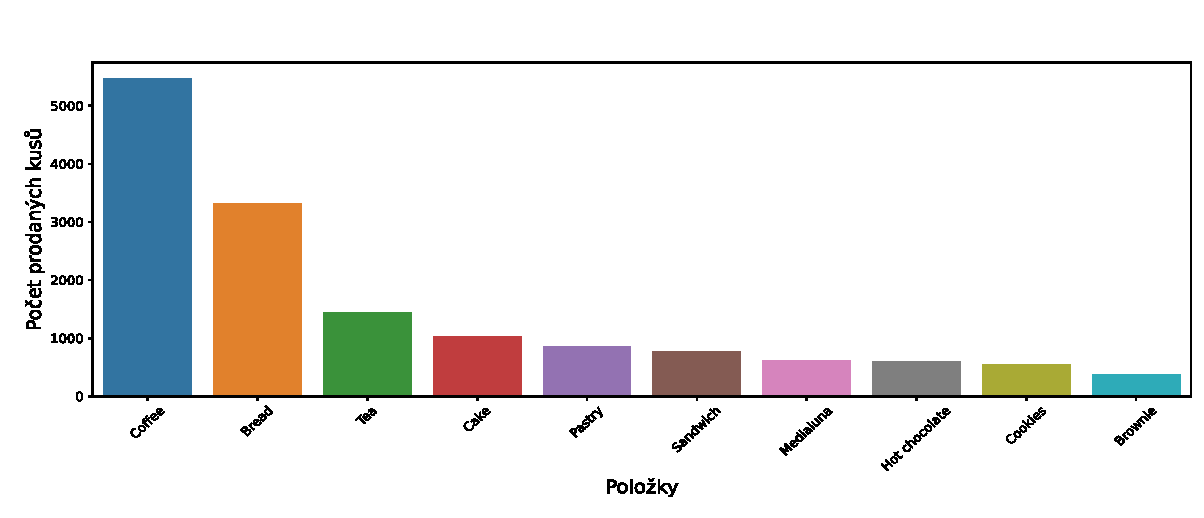
\includegraphics[width=\linewidth,height=2.7in]{obrazky/top10.pdf}\\[1pt]
  \caption{10 nejprodávanějších položek}
  \label{top10}
\end{figure*}

\subsection*{Dolování pravidel}
Jak bylo zmíněno v podkapitole \ref{knihovny_2}, tak \textit{scikit-learn} nenabízí žádnou možnost pro dolování asociačních pravidel. Proto pro zajímavost byla implementována vlastní varianta dolování asociačních pravidel pomocí využití algoritmu Apriori a jazyka Python.

Předtím než se začne proces dolování asociačních pravidel, bylo potřeba načtenou datovou sadu zpracovat do vhodné podoby. Načtena datová sada má podobu tabulky \ref{tab1}, kde je možné vidět prvních pět řádků struktury \verb|DataFrame|.

\begin{table}[]
    \centering
   \begin{tabular}{lrllll}
\toprule
{} &  Transaction &           Item &         date\_time & period\_day & weekday\_weekend \\
\midrule
0 &            1 &          Bread &  30-10-2016 09:58 &    morning &         weekend \\
1 &            2 &   Scandinavian &  30-10-2016 10:05 &    morning &         weekend \\
2 &            2 &   Scandinavian &  30-10-2016 10:05 &    morning &         weekend \\
3 &            3 &  Hot chocolate &  30-10-2016 10:07 &    morning &         weekend \\
4 &            3 &            Jam &  30-10-2016 10:07 &    morning &         weekend \\
\bottomrule
\end{tabular}
    \caption{Prvních pět řádků načtené datové sady}
    \label{tab1}
\end{table}

Pomocí funkce \verb|groupby()| z knihovny \textit{pandas} se transformuje tento \verb|DataFrame| na \verb|DataFrame|, který má podobu transakční tabulky. Nový vytvoření \verb|DataFrame| obsahuje dva sloupce: číslo transakce a položky. Tabulka \ref{tab2} zobrazuje prvních pět řádků transformované struktury \verb|DataFrame| do podoby transakční tabulky.

\begin{table}[]
    \centering
    \begin{tabular}{lrl}
\toprule
{} &  Transaction &                           Item \\
\midrule
0 &            1 &                        (Bread) \\
1 &            2 &                 (Scandinavian) \\
2 &            3 &  (Jam, Cookies, Hot chocolate) \\
3 &            4 &                       (Muffin) \\
4 &            5 &        (Bread, Pastry, Coffee) \\
\bottomrule
\end{tabular}
    \caption{Transakční tabulka}
    \label{tab2}
\end{table}

Položky v transakční tabulce byly uložené jako datový typ \verb|frozenset|, aby dále usnadnili práci s množinami. Dále transakční tabulka byla transformovaná na základní datovou strukturu jazyka Python \verb|dictionary| pro zjednodušení práce s daty.

Pro vytvoření frekventované množiny byla implementována funkce \verb|get_k_1_itemset()|. Tato funkce příjímá argument minimální podpory a vytváří první frekventovanou množinu, kde $k=1$. Tato množina obsahuje všechny položky, které splňují minimální podporu a z nich se dále vytvoří další kandidátní množina. 

Dále je implementován cyklus \verb|while|, kde funkce \verb|find_frequent_itemsets()| vrací aktuální frekventovánou množinu o velikosti $k$. Princip funkce je, že pokud existuje frekventovaná podmnožina, tak bude její nadmnožina taky frekventovaná. Cyklus se ukončí, když se nenajde žádná frekventovaná množina o velikosti $k$, která splňuje minimální podporu.

Potom co se generují všechny frekventované množiny, tak se z nich vytvářejí asociační pravidla ve tvaru $A \Rightarrow B$. Následně se počítá spolehlivost jednotlivých pravidel podle počtu výskytu v datové sadě.

Zde byla zvolena minimální podpora $1\%$, potom co bylo vyzkoušeno několik hodnot, aby vznikla nějaká asociační pravidla. Následuje ukázka devíti pravidel seřazené podle nejvyšší spolehlivosti. 
\begin{mdframed}
\begin{lstlisting}[language=Python]
Pravidlo 1: ['Toast'] -> Coffee | spolehlivost : 0.704
Pravidlo 2: ['Sandwich', 'Cake'] -> Coffee | spolehlivost : 0.677
Pravidlo 3: ['Pastry', 'Hot chocolate'] -> Coffee | spolehlivost : 0.667
Pravidlo 4: ['Sandwich', 'Soup'] -> Coffee | spolehlivost : 0.654
Pravidlo 5: ['Salad'] -> Coffee | spolehlivost : 0.626
Pravidlo 6: ['Cookies', 'Hot chocolate'] -> Coffee | spolehlivost : 0.614
Pravidlo 7: ['Cookies', 'Juice'] -> Coffee | spolehlivost : 0.603
Pravidlo 8: ['Cake', 'Hot chocolate'] -> Coffee | spolehlivost : 0.602
Pravidlo 9: ['Spanish Brunch'] -> Coffee | spolehlivost : 0.599
\end{lstlisting}   
\end{mdframed}

\subsubsection*{Mlxtend}
Jak bylo řečeno v podkapitole \ref{knihovny_2}, knihovna mlxtend nabízí dva algoritmy pro dolování asociačních pravidel, a to algoritmy Apriori a metoda FP-stromu. Zde si ukážeme implementaci obou algoritmů a následně je porovnáme z hlediska doby trvání jednolivých algoritmů. Metoda FP-stromu by měla být řádové rychlejší, protože negeneruje kandidátní množiny. 

Algoritmus Apriori je reprezentován funkci \verb|apriori()|, který na vstupu přijímá několik argumentů. Důležitým argumentem je \verb|min_support|, který reprezentuje minimální podporu pravidla. Pokud se nezvolí tento parametr, tak je předvolená hodnota nastavená na 0.5. Další poviný argument je datová sada ve speciálním formátu. 

Metoda FP-stromu je reprezentovaná funkci \verb|fpgrowth()|, která přijímá stejné argumenty jako výš uvedena funkce \verb|apriori()|. 

Nejdříve je potřeba transformovat naši datovou sadu, která má tvar tabulky \ref{tab1}, do podoby, která má tvar $MxN$, kde $M$ je počet řádků, které reprezentují jednotlivé transakce, a kde $N$ jsou jednotlivé položky, která pekárna prodává a hodnoty této tabulky jsou \verb|True| v případě, že je položka součástí této transakce, jinak je hodnota \verb|False|. Tuto podobu datové sady přijímají na vstupu obě funkce pro vytvoření frekventovaných množín.

Jak už bylo zjištěno z vlastní implementace, zde bude taky zvolena minimální podpora $1\%$.
\begin{mdframed}
\begin{lstlisting}[language=Python]
#nacteni funkci z knihovny
from mlxtend.frequent_patterns import apriori, fpgrowth

#vytvoreni frekventovanych mnozin pomoci Apriori
fitems = apriori(xtend_data, min_support = 0.01, use_colnames=True)

#vytvoreni frekventovanych mnozin pomoci FP-growth
fitems_fpg = fpgrowth(xtend_data, min_support = 0.01, use_colnames=True)
\end{lstlisting}   
\end{mdframed}

Obě funkce vrací \verb|DataFrame|, který obsahuje frekventované množiny a je možné ho upravit libovolně pomocí funkce z knihovny \textit{pandas}.

Ten se dále předá funkci \verb|association_rules()|, která přijímá i další argumenty například metriky, podle kterých se budou tvořit asociační pravidla a minimalní hodnotu této metriky. My zde necháme předvolenou hodnotu metriky, která je spolehlivost a jen upravíme minimalní hodnotu této metriky na 0.3.

\begin{mdframed}
\begin{lstlisting}[language=Python]
#nacteni funkci z knihovny
from mlxtend.frequent_patterns import association_rules

#vytvoreni pravidel pomoci algoritmu Apriori
rules = association_rules(fitems, min_threshold=0.3)

#vytvoreni pravidel pomoci algoritmu FP-grow
rules_fpg = association_rules(fitems_fpg, min_threshold=0.3)
\end{lstlisting}   
\end{mdframed}

Výsledek asociačních pravidel obou algoritmů je totožný a je vrácen v podobě \verb|DataFrame|, který je upraven, aby zobrazil pravidla sestupně podle metriky spolehlivosti a má podobu tabulky \ref{tab3}, kde jsou první devět pravidel.

\begin{table}[]
    \centering
    \small
    \begin{tabular}{lllrrrr}
\toprule
{} &       antecedents & consequents &  antecedent support &  consequent support &   support &  confidence \\
\midrule
0 &           (Toast) &    (Coffee) &   0.033597 &            0.478394 &  0.023666 &    0.704403 \\
1 &  (Spanish Brunch) &    (Coffee) &   0.018172 &            0.478394 &  0.010882 &    0.598837 \\
2 &       (Medialuna) &    (Coffee) &   0.061807 &            0.478394 &  0.035182 &    0.569231 \\
3 &          (Pastry) &    (Coffee) &   0.086107 &            0.478394 &  0.047544 &    0.552147 \\
4 &       (Alfajores) &    (Coffee) &   0.036344 &            0.478394 &  0.019651 &    0.540698 \\
5 &           (Juice) &    (Coffee) &   0.038563 &            0.478394 &  0.020602 &    0.534247 \\
6 &        (Sandwich) &    (Coffee) &   0.071844 &            0.478394 &  0.038246 &    0.532353 \\
7 &            (Cake) &    (Coffee) &   0.103856 &            0.478394 &  0.054728 &    0.526958 \\
8 &           (Scone) &    (Coffee) &   0.034548 &            0.478394 &  0.018067 &    0.522936 \\
\bottomrule
\end{tabular}
    \caption{První devět pravidel knihovny mlxtend}
    \label{tab3}
\end{table}

Když se provede časově porovnání algoritmů, v tomto případě Apriori je mnohem rychlejší než metoda FP-stromu.

\begin{mdframed}
\begin{lstlisting}[language=Python]
>>> %timeit -n 100 -r 10 apriori(xtend_data, min_support = 0.01)
>>> %timeit -n 100 -r 10 fpgrowth(xtend_data, min_support = 0.01)
\end{lstlisting}   
\end{mdframed}

\subsubsection*{PyCaret}
Knihovna PyCaret nabízí jen algoritmus Apriori. Nejdříve se zavolá funkce \verb|setup()|, která automaticky zpracuje vstupní datovou sadu \ref{tab1}. Pomocí argumentů určíme, jaký sloupec reprezentuje transakci a jaký sloupec reprezentuje položky, z kterých se bude tvořit asociační pravidla.

\begin{mdframed}
\begin{lstlisting}[language=Python]
#nacteni funkci z knihovny
from pycaret.arules import *

exp = setup(data=df, transaction_id='Transaction', item_id='Item')
\end{lstlisting}   
\end{mdframed}

Poté se zavolá funkce \verb|create_model()|, kde se určí minimální podpora, metrika a práh této metriky. V tomto případě minimální podpora bude $1\%$, metrika je spolehlivost a práh bude hodnota 0.3.

\begin{mdframed}
\begin{lstlisting}[language=Python]
model1 = create_model(metric="confidence", 
                      min_support=0.01, 
                      threshold=0.3)
\end{lstlisting}   
\end{mdframed}

Výsledek, který vrací tato funkce, je totožný s výsledkem knihovny \textit{mlxtend} a má tedy podobu tabulky \ref{tab3}. Pomocí funkce \verb|plot_model()| je možné asociační pravidla zobrazit. Pravidla je možné vidět na obrázku \ref{pravidla} ve 2D grafu. Pokud změníme argument \verb|plot| na 3d, tak se asociační pravidla zobrazí ve 3D grafu. Existuje ještě funkce \verb|get_rules()|, která je kombinaci předchozích dvou funkci.

\begin{figure*}[h]\centering
  \centering
  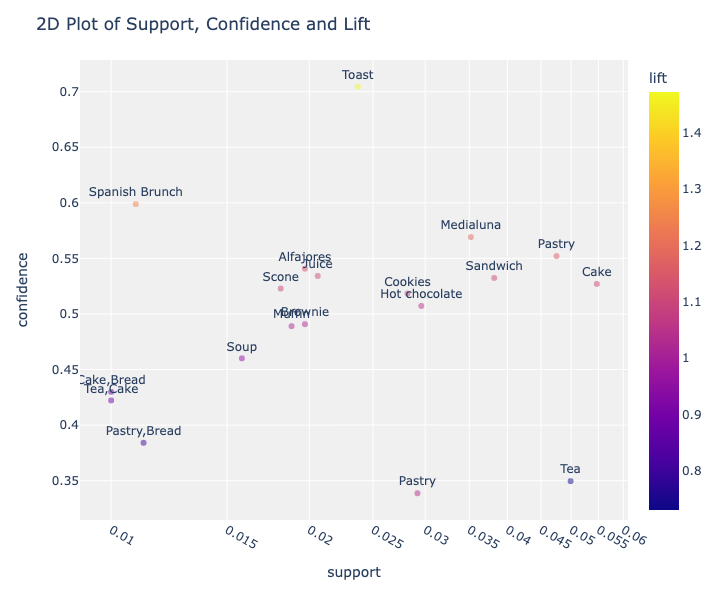
\includegraphics[width=\linewidth,height=4.7in]{obrazky/newplot2.png}\\[1pt]
  \caption{Asociační pravidla}
  \label{pravidla}
\end{figure*}

\subsection*{Zhodnocení experimentu}
Z vytvořených asociačních pravidel se dá vyvodit, že nejdůležitější produktem této pekárny je káva. Když klient kupoval něco k snědku, tak vždycky k tomu dokupoval kávu. Až v $70\%$ případů lidí, kteří kupovali toast, tak k tomu koupili i kávu. V budoucnu by mohla tato pekárna například udělat nějakou akci pro toast a kávu. 

Z hlediska vygenerovaných asociačních pravidel knihovny \textit{mlxtend} a \textit{PyCaret} dosahli stejného výsledků. Vlastní ímplementace se shoduje v pravidlech, které byly generované z frekventovaných množin, kde $k=2$, například: $Toast \Rightarrow Coffee$ se spolehlivosti $70\%$ a $Spanish\ Brunch \Rightarrow Coffea$ se spolehlivosti $59\%$. Vlastní implementace našla 27 frekventovaných množín, kde $k=3$. Algoritmus Apriori z \textit{mlxtend} našlo jen 3 frekventované množiny, kde $k=3$ a metoda FP-stromu ani jednu. Toto může být způsobeno nedokonalou optimalizaci algoritmů. 

Pokud chceme vyřešit úlohu, kde je potřeba vytvořit asociační pravidla, tak máme na výběr ze třech možnosti, a to využít buď knihovny \textit{mlxtend} nebo \textit{PyCaret}, anebo vlastní implementací. Mlxtend oproti PyCaret nabízí metodu FP-stromu, ale výhoda knihovny PyCaret je jednoduché rozhraní, které nabízí k vytvoření asociačních pravidel.

\section{Klasifikace}
Tento experiment je zaměřený na ukázku klasifikace pomocí různých metod s využitím jednotlivých knihoven prezentované v podkapitole \ref{knihovny_2}. Půjde tu hlavně o rozhodovací stromy, model náhodného lesa, bayesovskou klasifikaci, neuronové sítě a k-nejbližších sousedů. Experiment bude implementován nad datovou sadou, která dělí rýžová zrnka do dvou tříd. Jedná se tedy o binární klasifikaci. Cílem bude sledovat, jak se jednotlivé knihovny tímto úkolem vypořádají a zároveň změřit přesnost jednotlivých algoritmů z jednotlivých knihoven. 

V první části se představí datová sada. Následně bude popsán proces vytvoření klasifikačního modelu podle algoritmu, které jsou k dispozici z jednotlivých knihoven. V závěru bude následovat zhodnocení experimentu.

\subsection*{Datová sada rýžových zrn}
Datová sada pro tento experiment je dostupná online\footnote{\url{https://www.kaggle.com/datasets/muratkokludataset/rice-dataset-commeo-and-osmancik?resource=download}} a obsahuje 3810 snímků rýžových zrn, které byly získané pomocí počítačového vidění. Tyto snímky byly zpracovány. Na základě tohoto pro každé zrnko bylo získáno 7 morfologických znaků, které klasifikuje tyto zrnka do dvou možných druhů rýže a to \textbf{Cammeo} nebo \textbf{Osmancik}. Jednotlivé morfologické znaky popisují následující údaje: 

\begin{itemize}
    \item \textbf{Obsah} -- vrátí počet pixelů v rámci hranic rýžového zrna.
    \item \textbf{Obvod} -- vypočítá obvod výpočtem vzdálenosti mezi pixely kolem hranic rýžových zrn.
    \item \textbf{Délka hlavní osy} -- udává nejdelší čáru, kterou lze na rýžovém zrnu nakreslit, tj. vzdálenost hlavní osy.
    \item \textbf{Délka vedlejší osy} -- nejkratší čára, která může být nakreslena na zrnu rýže, tj. malá vzdálenost osy.
    \item \textbf{Excentricita} -- měří, jak kulatá je elipsa, která má stejné momenty jako zrnko rýže.
    \item \textbf{Konvexní oblast} -- vrátí počet pixelů nejmenší konvexní slupky v oblasti tvořené zrnem rýže.
    \item \textbf{Rozsah} -- vrátí poměr oblasti tvořené zrnem rýže k pixelům ohraničujícího rámečku.
\end{itemize}

Protože soubor, v kterém se nachází tato datovová sada, je ve formátu xlsx, tak pro jeho načtení použijeme další možnou funkci z knihovny \textit{pandas}, kterou lze vidět na následující ukázce: 

\begin{mdframed}
\begin{lstlisting}[language=Python]
#nacteni dat z xlsx souboru
df = pd.read_excel("datasets/Rice_Cammeo_Osmancik.xlsx")
\end{lstlisting}   
\end{mdframed}

Tuto datovou sadu můžeme prozkoumat pomocí různých funkcí knihovny \textit{pandas}, které byly zmíněné v podkapitole \ref{asociacni-pravidla}. Datová sada neobsahuje žádné chybějící hodnoty. Dále si můžeme zobrazit rozložení hodnot jednotlivých atributů této datové sady. Výsledek je možné vidět na obrázku \ref{hodnoty-klasifikace}.

\begin{figure*}[h]\centering
  \centering
  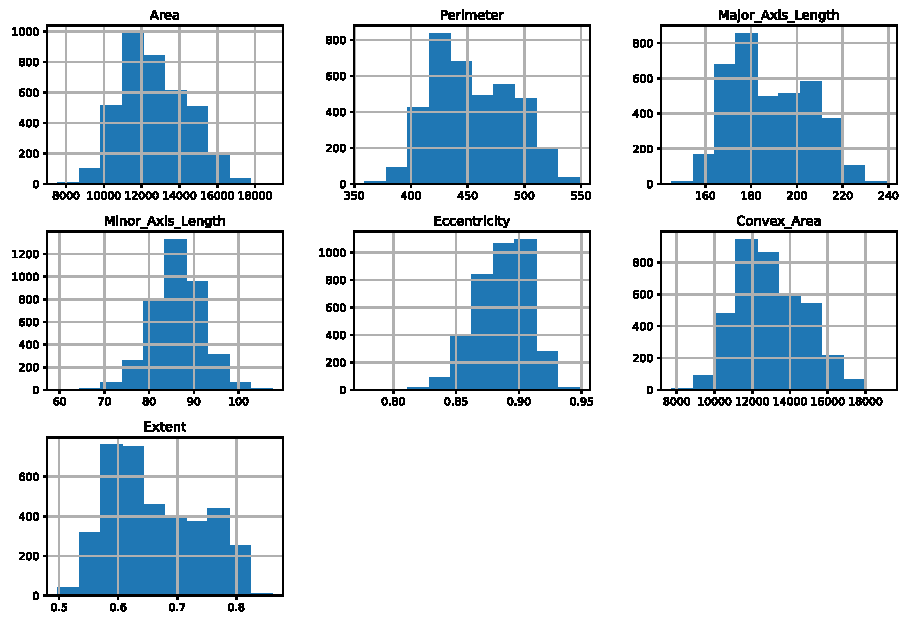
\includegraphics[width=\linewidth,height=4.7in]{obrazky/hodnoty-klasifikace.pdf}\\[1pt]
  \caption{Rozložení hodnot jednotlivých atributů}
  \label{hodnoty-klasifikace}
\end{figure*}

\subsection*{Klasifikace pomocí knihovny scikit-learn}

Nejdřív se datová sada rozdělí do dvou proměnných. Proměna \verb|X| obsahuje 7 morfologických znaků rýžového zrnka a proměna \verb|y| obsahuje třídu, do kterého budeme klasifikovat zrnko. 

Dále je potřeba rozdělit datovou sadu na trénovací a testovací (validační) množinu. Toto se realizuje pomocí funkce z knihovny \textit{scikit-learn}. Využití této funkce lze vidět na následující ukázce. 

\begin{mdframed}
\begin{lstlisting}[language=Python]
#nacteni funkce z knihovny
from sklearn.model_selection import train_test_split

#rozdeleni datove sady na trenovaci a testovaci mnozinu
X_train, X_test, y_train, y_test = train_test_split(X,y, random_state=14)
\end{lstlisting}   
\end{mdframed}

Dále se vytvoří modely rozhodovacího stromu, náhodného lesa a bayesovské klasifikace. Jejích tvorba je prezentována na následující ukázce. 


\begin{mdframed}
\begin{lstlisting}[language=Python]
#nacteni funkce z knihovny
from sklearn.tree import DecisionTreeClassifier

#tvorba rozhodovaciho stromu
dt_clf = DecisionTreeClassifier()

from sklearn.ensemble import RandomForestClassifier

#tvorba nahodneho lesa
rf_clf = RandomForestClassifier

from sklearn.naive_bayes import GaussianNB

#tvorba bayesovske klasifikace
nb_clf = GaussianNB()
\end{lstlisting}   
\end{mdframed}

Po tvorbě rozhodovacího stromu je možné si model zobrazit pomocí funkce \verb|plot_tree()|, který je možné vidět na obrázku \ref{strom-scikit}.

\begin{figure*}[h]\centering
  \centering
  \includegraphics[width=\linewidth,height=4.7in]{obrazky/decistion_tree.pdf}\\[1pt]
  \caption{Vizualizace rozhodovacího stromu knihovny scikit-learn}
  \label{strom-scikit}
\end{figure*}

Každý model následně je trénovan pomocí funkce \verb|fit()| předáním trénovací množiny, která se skládá ze dvou proměnných \verb|X_train| a \verb|y_train|. Klasifikace je následně vykonána funkci \verb|predict()|, která přijímá na vstupu testovací množinu. 

Pro modely neuronových sítí a $k$--nejbližších sousedů je dobré data normalizovat, aby učení bylo rychlejší a přesnější. Normalizace je realizována pomocí jednoduché funkce nad hodnoty atributů, které reprezentují 7 morfologických znaků jednotlivých rýžových zrn. V tomto experimentu hodnoty budou normalizované do intervalu 0 až 1.

\begin{mdframed}
\begin{lstlisting}[language=Python]
#nacteni funkce z knihovny
from sklearn.preprocessing import normalize

#normalizace
X_normalized = normalize(X, norm='max')
\end{lstlisting}   
\end{mdframed}

Jednotlivé modely se vytvoří pomocí patřičných tříd. V případě modelu neuronové sítě
třída \verb|MLPClassifier()| přijímá několik parametrů. Jeden z parametrů říká kolik bude neuronu ve skryté vrstvě. Zde je hodnota 4, potom co se zaokrouhlila na základě předpisů \ref{predpis}:

\begin{equation}
    \sqrt{m*n}
    \label{predpis}
\end{equation}

kde $m$ počet neuronu ve vstupní vrstvě a $n$ je počet neuron ve výstupní vrstvě.

\begin{mdframed}
\begin{lstlisting}[language=Python]
#nacteni funkce z knihovny
from sklearn.neural_network import MLPClassifier

mlp_clf = MLPClassifier(hidden_layer_sizes=(4,), random_state=14)

#nacteni funkce z knihovny
from sklearn.neighbors import KNeighborsClassifier

knn_clf = KNeighborsClassifier()
\end{lstlisting}   
\end{mdframed}

Trénování a klasifikace probíhá stejně jako u výše zmíněných modelu. 

Dále tyto všechny modely je možné zhodnotit pomocí funkce \verb|accuracy_score()| z modulu \verb|sklearn.metrics|. Funkce vrací hodnotu mezi 0 a 1, která udává s jakou přesností model klasifikoval. Pokud by hodnota byla 1, znamenalo by to, že všechny záznamy byly správně klasifikované. Výsledky v procentech jednotlivých modelů je možné vidět v tabulce \ref{tab4}.

\begin{table}[]
    \centering
    \begin{tabular}{llr}
\toprule
{} &                    Model &      Skore \\
\midrule
1 &             Náhodné lesy &  91.920252 \\
2 &  Bayesovská klasifikace &  91.605456 \\
3 &       Rozhodovací stromy &  88.457503 \\
4 &    K–nejbližších sousedů &  88.457503 \\
5 &           Neuronové sítě &  56.663169 \\
\bottomrule
\end{tabular}
    \caption{Výsledky v procentech jednotlivých modelů knihovny scikit-learn}
    \label{tab4}
\end{table}

Další funkci, která zobrazuje přesnost klasifikátoru je \verb|confusion_matrix()|, která vytváří tzv. konfúzní matici. Tato matice se skládá z $n$ řádku a $n$ sloupců. Řádky a sloupce reprezentují kategorie, do kterých byly testovací hodnoty klasifikovány. Jednotlivé buňky obsahují počet hodnot, které realně patří do dané třídy a byli klasifikátorem přiřazeny do stejné nebo jiné třídy. Výsledky této funkce je možné vidět na obrázku \ref{konfuznimatice}

\begin{figure*}[h]\centering
  \centering
  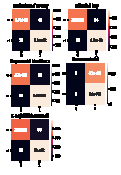
\includegraphics[width=\textwidth,height=5.7in]{obrazky/modely.pdf}\\[1pt]
  \caption{Konfúzní matice jednotlivých modelů knihovny scikit-learn}
  \label{konfuznimatice}
\end{figure*}

\subsection*{Klasifikace pomocí knihovny mlxtend}
Knihovna nabízí 3 varianty modelu neuronových sítí. Nejdřív zpracujeme datovou sadu do vhodné podoby. Hodnoty atributů je potřeba normalizovat stejně jako v případě implementace pomocí knihovny \textit{scikit-learn}.  

Normalizace je realizována pomocí funkce \verb|minmax_scaling()|. Dále data rozdělíme na trénovací a testovací množinu pomocí funkce z knihovny \textit{scikit-learn}, protože zde neexistuje obdobná alternativa.

Následně vytvoříme jednotlivé modely. 

\begin{mdframed}
\begin{lstlisting}[language=Python]
#nacteni trid z knihovny
from mlxtend.classifier import Perceptron, Adaline, MultiLayerPerceptron

ppn = Perceptron()
nn1 = MLP(hidden_layers=[4])
ada = Adaline()
\end{lstlisting}   
\end{mdframed}

Jednotlivé modely jsou trénované pomocí funkce \verb|fit()| a následná klasifikace probíhá pomocí funkce \verb|predict()|. Jedná se o stejný postup jako v případě knihovny \textit{scikit-learn}. 

Pro vyhodnocení jsou k dispozici opět obdobné funkce, které nabízí knihovna \textit{scikit-learn}. Výsledky přesnosti klasifikátoru lze vidět v tabulce \ref{tab5}. Konfúzní matice jsou na obrázku \ref{konfuznimaticex}

\begin{table}[]
    \centering
    \begin{tabular}{llr}
\toprule
{} &                    Model &      Skore \\
\midrule
1 &             Adaline &  92.864637 \\
2 &             Perceptron &  85.72927 \\
3 &  MultiLayerPerceptron &  56.663168 \\
\bottomrule
\end{tabular}
    \caption{Výsledky v procentech jednotlivých modelů knihovny mlxtend}
    \label{tab5}
\end{table}

\begin{figure*}[h]\centering
  \centering
  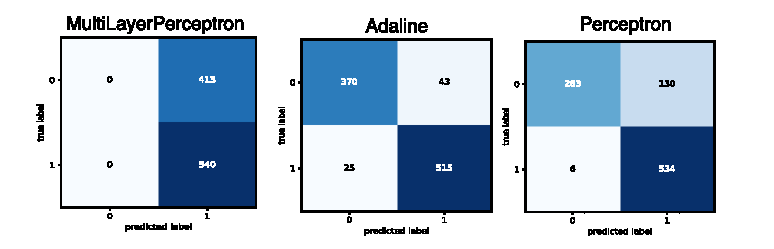
\includegraphics[width=\textwidth,height=2.7in]{obrazky/mlp_mx.pdf}\\[1pt]
  \caption{Konfúzní matice jednotlivých modelů knihovny mlxtend}
  \label{konfuznimaticex}
\end{figure*}

\subsection*{Klasifikace pomocí knihovny PyCaret}
Tato knihovna nabízí velice jednoduché rozhraní pro implementaci této úlohy. 
Pomocí funkce \verb|setup()|, které předáme jako argument datovou sadu, kterou jsme načetli funkci z knihovny \textit{pandas} a nastavíme, který sloupec určuje třídu, do které se bude klasifikovat přes argument \verb|target|. Tato funkce automatický předzpracuje data, a potom rozdělí data na trénovací a testovací množinu.

Dále vytvoříme model funkci \verb|create_model()|, kde určíme podle jakého algoritmu se má tento model vytvořit. Funkce dále automatický trénuje model, pak klasifikuje testovací množinu a nakonec vrací přesnost klasifikátoru jako výsledek. 

\begin{mdframed}
\begin{lstlisting}[language=Python]
#nacteni funkci z knihovny
from pycaret.classification import *

#predzpracovani dat
exp = setup(data=df, target='Class', silent=True)

#vytvoreni, trenovani a testovani rozhodovaciho stromu
dt = create_model('dt', cross_validation=False)

#vytvoreni, trenovani a testovani nahodneho lesa
rf = create_model('rf', cross_validation=False)

#vytvoreni, trenovani a testovani bayesovske klasifikaci
nb = create_model('nb', cross_validation=False)

#vytvoreni, trenovani a testovani neuronove site
mlp = create_model('mlp', cross_validation=False)

#vytvoreni, trenovani a testovani k-nejblizsich sousedu
knn = create_model('knn', cross_validation=False)
\end{lstlisting}   
\end{mdframed}
Existuje ještě funkce \verb|plot_model()|, kde předáním různých argumentů je možné vykreslit různé grafy. Například při vytvoření rozhodovacího stromu lze tuto funkci využít pro zobrazení tohoto modelu. Pomocí této funkce lze též vykreslit konfúzní matice.

\begin{mdframed}
\begin{lstlisting}[language=Python]
plot_model(dt, plot = 'tree')
\end{lstlisting}   
\end{mdframed}

Výsledky přesnosti klasifikátoru této knihovny lze vidět v tabulce \ref{tab6} a konfúzní matice jsou na obrázku \ref{konfuznimaticepycaret}.

\begin{table}[]
    \centering
    \begin{tabular}{llr}
\toprule
{} &                    Model &      Skore \\
\midrule
1 &             Náhodné lesy &  92.22 \\
2 &  Bayesovská klasifikace &  91.35 \\
3 &       K–nejbližších sousedů & 89.60 \\
4 &    Rozhodovací stromy &  89.16 \\
5 &           Neuronové sítě &  72.29 \\
\bottomrule
\end{tabular}
    \caption{Výsledky v procentech jednotlivých modelů knihovny PyCaret}
    \label{tab6}
\end{table}

\begin{figure*}[h]\centering
  \centering
  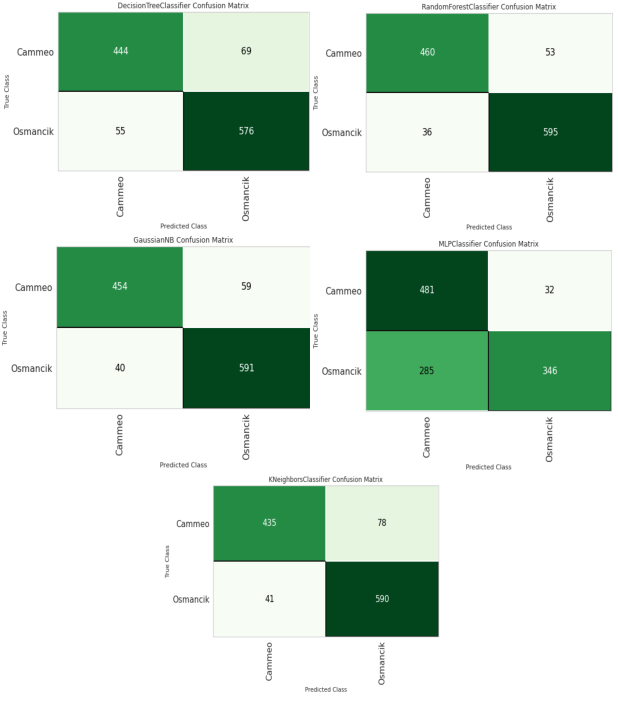
\includegraphics[width=4in,height=4.7in]{obrazky/pycaretklf.pdf}\\[1pt]
  \caption{Konfúzní matice jednotlivých modelů knihovny PyCaret}
  \label{konfuznimaticepycaret}
\end{figure*}

\subsection*{Zhodnocení experimentu}
Lze vidět, že z hlediska nabízeních algoritmů knihovny scikit-learn a PyCaret pokrývají všechny prezentované klasifikační algoritmy z kapitoly \ref{metody}. 

Modely knihovny PyCaret jsou o něco přesnější než ty vytvořené knihovnou scikit-learn. V obou případech nejlepší model byl náhodný les a následně za ním bayesovký klasifikátor. Ve všech případech nejhorší model byl vícevrstvový Perceptron (MLP). Celkově nejlepší model byl uměly neuron Adaline z knihovny mlxtend. 

Je třeba dodat, že modely vytvořené knihovnou scikit-learn a PyCaret můžou byt ještě optimalizované, aby dosáhli lepšího výsledku.

\section{Shluková analýza}
\label{shlukovanalyza}
Poslední experiment je zaměřen na ukázku shlukování založeného na rozdělování, hierarchického shlukování a shlukování založeného na hustotě. Jako zdroj dat pro shlukování je vybrána datová sada o tučňácích žijících na souostroví Palmer Archipelago na Antakrtidě. Cílem bude sledovat, jak se jednotlivé knihovny tímto
úkolem vypořádají. 

V první části se představí datová sada. Následně po ní následuje ukázka jednotlivých technik shlukování, které jsou k dispozici z jednotlivých knihoven.
V závěru bude následovat zhodnocení experimentu.

\subsection*{Datová sada o tučňácích žijících na souostroví Palmer Archipelag}
Tato online\footnote{\url{https://www.kaggle.com/datasets/parulpandey/palmer-archipelago-antarctica-penguin-data?select=penguins_size.csv}} dostupná datová sada byla vytvořená doktorkou Kristen Gorman a výzkumnou stanici Palmer na Antarktidě. Datová sada obsahuje celkem 344 záznamu. Každý záznam reprezentuje konkrétní tučňák v podobě 6 atributu jako pohlaví, váha, míry zobáku a ostrov, na kterém žijí. Atribut \verb|species| má 3 hodnoty: Adélie, Gentoo, Chinstrap. Jedná se o druh, do kterého patří jednotlivé záznamy. V tomto experimentu se tento atribut odstraní.

Po načtení datové sady a její analýzu bylo zjištěno, že obsahuje nevalidní a chybějící hodnoty, které je potřeba odstranit. Dále datová sada má 2 kategorické atributy: pohlaví a ostrov. Hodnoty těchto atributu nahradíme za kvantitativní hodnoty.

\begin{mdframed}
\begin{lstlisting}[language=Python]
island_map = {"Biscoe": 0, "Dream": 1, "Torgersen": 2}
sex_map = {"MALE": 0, "FEMALE": 1}
df = df.applymap(lambda s: island_map.get(s) if s in island_map else s)
df = df.applymap(lambda s: sex_map.get(s) if s in sex_map else s)
\end{lstlisting}   
\end{mdframed}

Pro lepší výsledky shlukování je potřeba hodnoty normalizovat, aby každy atribut měl stejnou váhu. Normalizace probíhá stejně jako v případě klasifikace pomocí neuronových sítí, kde hodnoty jsou z intervalu 0 až 1.

\subsubsection*{Scikit-learn}
V této knihovně je nejběžnější technika shlukování založené na rozdělení reprezentovaná třídou \verb|KMeans()| . Tato třída přijímá na vstupu počet cílových shluků, který je potřeba zjistit. 

Pro zjištění počtu využijeme tuto třídu. Tato třída obsahuje atribut \verb|inertia_|, který udává součet vzdáleností vzorků k jejich nejbližšímu středu shluku. Tato hodnota se může interpretovat jako nepřesnost shlukování. Tato nepřesnost je otestována pro 1 až 14 shluků, kde je možné vidět výsledek na obrázku \ref{k-err}. Optmimální hodnota pro cílový počet shluků je 3, protože jde o hraniční hodnotu, od které se nepřesnost shlukování moc nesnižuje.

\begin{figure*}[h]\centering
  \centering
  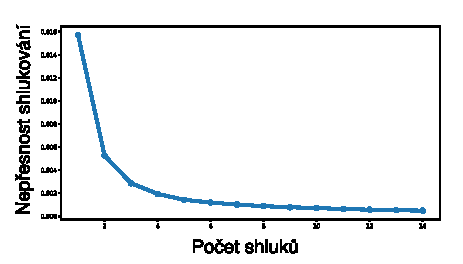
\includegraphics[width=\textwidth,height=2.7in]{obrazky/k-err.pdf}\\[1pt]
  \caption{Nepřesnost shlukování v závislosti na počtu shluků}
  \label{k-err}
\end{figure*}

Po výběru počtu shluků je možné realizovat shlukovou analýzu. 

\begin{mdframed}
\begin{lstlisting}[language=Python]
#nacteni tridy z knihovny
from sklearn.cluster import KMeans

kmeans = KMeans(n_clusters=3)
kmeans_clusters = kmeans.fit_predict(X_normalized)
\end{lstlisting}   
\end{mdframed}
Pomocí funkce \verb|fit_predict()| se vypočítají středy shluků a každý vzorek je umístěn do shluku. Výsledné shluky je možné zobrazit pomocí knihoven \textit{seaborn} a \textit{matplotlib} na různých atributech. Ukázka je na obrázku \ref{k-means}, kde za atributy byly zvolené míry zobáku a porovnává se s původní datovou sadou. Pro správnost přesnosti shlukování můžeme využít funkce \verb|value_counts()| knihovny \textit{pandas}. 

\begin{figure*}[h]\centering
  \centering
  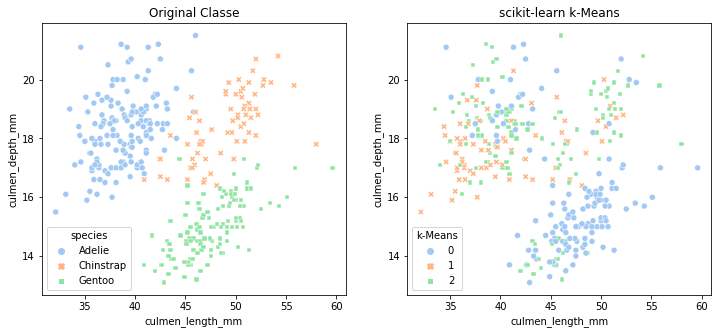
\includegraphics[width=4.2in,height=2.2in]{obrazky/kmeans.png}\\[1pt]
  \caption{Výsledek shlukování k-means knihovny scikit-learn}
  \label{k-means}
\end{figure*}

Hierarchické shlukování je zastoupeno třídou \verb|AgglomerativeClustering()|. Pomocí vykreslení dendogramu je možné stanovit práh vzdálenosti mezi shluky a jako kriterium bylo stanovené spojení \verb|average|. Toto kritérium stanovuje, že vzdálenost mezi dvěma shluky je vypočitaná jako průměr vzdáleností mezi vzorky jednoho a druhého shluku.

\begin{mdframed}
\begin{lstlisting}[language=Python]
#nacteni tridy z knihovny
from sklearn.cluster import AgglomerativeClustering

agg1 = AgglomerativeClustering(linkage='average', 
                               distance_threshold=0.008, n_clusters=None)
\end{lstlisting}   
\end{mdframed}
Pro vyhodnocení a zobrazeni výsledků je použit stejný postup jako u \textbf{k-means}. 

Posledním typem shlukování je shlukování založené na hustotě. Představitelem této skupiny shlukování je metoda DBSCAN, který je zde reprezentována třídou \verb|DBSCAN()|. Rozdíl této metody oproti ostatním je, že na vstupu je nutné zadat místo počtu shluků dva parametry: \verb|eps| (velikost okolí) a \verb|min_samples| (minimální počet bodů v okolí). Parametry je třeba předem zjistit. Ke zjištění optimální hodnoty okolí je možné využít třídu \verb|NearestNeighbors()| pro získání vzdálenosti $k$ nejbližších sousedů k daným bodům. Výsledek můžeme vykreslit v podobě grafu, který je na obrázku \ref{epsilon}. Optimální hodnota eps je stanovena na základě místa v grafu, kde vzdálenost k-nejbližších sousedů začíná prudce růst. Potom se vytvoří model, který se volá s optimálními hodnotami parametrů. 

\begin{figure*}[h]\centering
  \centering
  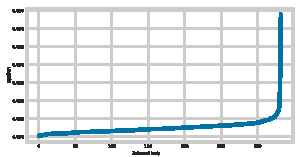
\includegraphics[width=\textwidth,height=2.7in]{obrazky/epsilon-db.pdf}\\[1pt]
  \caption{Výsledek pro optimalní okolí}
  \label{epsilon}
\end{figure*}

\begin{mdframed}
\begin{lstlisting}[language=Python]
#nacteni tridy z knihovny
from sklearn.cluster import DBSCAN

dbscan = DBSCAN(eps=0.0015, min_samples=24)
#trenovani a zarazeni vzorku
dbscan_clusters = dbscan.fit_predict(X_normalized)
\end{lstlisting}   
\end{mdframed}
Následně probíhá vyhodnocení této metody stejně jako v předchozích příkladech.

\subsubsection*{Mlxtend}
Jediný algoritmus, který nabízí tato knihovna pro shlukování, je metoda \textbf{k-Means}. Implementace je realizována pomocí třídy \verb|Kmeans()|, která přijímá jako parametr počet shluků, do kterých budeme zařazovat data. Využijeme znalost z předchozí části experimentu, a zde použijeme už rovnou hodnotu 3 pro počet shluků. 

\begin{mdframed}
\begin{lstlisting}[language=Python]
#nacteni tridy z knihovny
import mlxtend.cluster

#vytvoreni modelu, trenovani a zarazeni
kmeans_mlxtend = mlxtend.cluster.Kmeans(k=3)
kmeans_mlxtend.fit(X_normalized)
kmeans_mlxtend_clusters = kmeans_mlxtend.predict(X_normalized)
\end{lstlisting}   
\end{mdframed}

Výsledek shlukování je zde úplně stejný jako v případě využití metody k-means z knihovny \textit{scikit-learn}.

\subsubsection*{PyCaret}
Pro shlukovou analýzu tato knihovna nabízí stejně algoritmy jako knihovna \textit{scikit-learn}. Pro zpracování datové sady je opět k dispozici funkce \verb|setup()|, které se předá datová sada, nastaví se argument \verb|normalize| na hodnotu \verb|True|, aby data byla normalizovaná. Jako poslední argument se nastaví
atribut, který se bude ignorovat, aby se mohlo shlukovat bez něho. V tomto případě
bude se jednat o atribut \verb|species|. 

Vytvoření modelu je realizováno pomocí funkce \verb|create_model()|, kde se určí metodu shlukování, která bude použitá. 

\begin{mdframed}
\begin{lstlisting}[language=Python]
#nacteni funkci z knihovny
from pycaret.clustering import *

exp = setup(df, normalize=True, ignore_features=['species'], silent=True)

k_means = create_model('kmeans')
hclust = create_model('hclust')
dbscan = create_model('dbscan')
\end{lstlisting}   
\end{mdframed}

Dále pomocí funkce \verb|plot_model()|, můžeme vykreslit různé typy grafu. Například pro k-means lze vykreslit graf typu \verb|elbow|, který reprezentuje nepřesnost shlukování. Zde je optmimální hodnota pro cílový počet shluků je 5, jak je vidět na obrázku \ref{kmeanspycaret}. 

\begin{figure*}[h]\centering
  \centering
  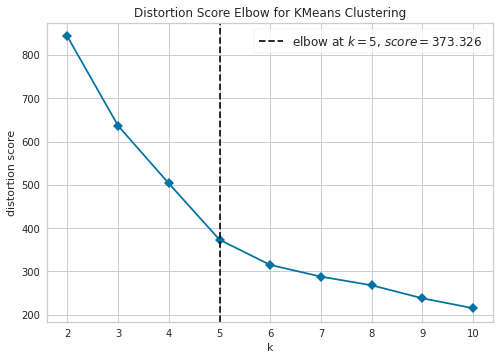
\includegraphics[width=4in,height=2.7in]{obrazky/pycaretkmeans.png}\\[1pt]
  \caption{Nepřesnost shlukování v závislosti na počtu shluků}
  \label{kmeanspycaret}
\end{figure*}

Dále lze vykreslit výsledné shluky nastavením argumentu \verb|plot| na klíčové slovo\verb|cluster|. Výsledek lze vidět na obrázku \ref{kmeanspycaretclusters}.

\begin{figure*}[h]\centering
  \centering
  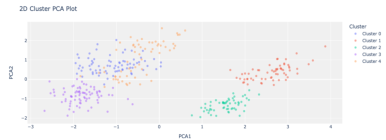
\includegraphics[width=\linewidth,height=2.0in]{obrazky/clusterspycaret.pdf}\\[1pt]
  \caption{Výsledek shlukování k-means knihovny PyCaret}
  \label{kmeanspycaretclusters}
\end{figure*}

V případě hierarchického shlukování implementace knihovny PyCaret vrací stejné výsledky
jako implementace k-means. Oba dva algoritmy rozdělují data do 5 shluků, ale toto rozdělení není přesné, protože jsou jenom 3 druhy tučňáků. 

Při implementaci shlukování založené na hustotě pomocí metody DBSCAN jsou data rozdělena do výsledných 9 shluků a vizualizace možné vidět na obrázku \ref{dbscanpycaretclusters}.

\begin{figure*}[h]\centering
  \centering
  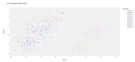
\includegraphics[width=\linewidth,height=2.0in]{obrazky/dbscanpycaret.pdf}\\[1pt]
  \caption{Výsledek shlukování DBSCAN knihovny PyCaret}
  \label{dbscanpycaretclusters}
\end{figure*}

\subsection*{Zhodnocení experimentu}
Knihovna mlxtend nabízí jediný algoritmus k-means pro řešení shlukovcích úloh. Tento algoritmus dosahuje stejného výsledků jako algoritmus k-means knihovny scikit-learn. Algoritmy zařadili 321 z 333 ($ 96,37 \%$) záznamu správně. Hierarchického shlukování z knihovny scikit-learn vrátil jako výsledek 4 shluky, ale v jednom z shluku nachází jenom jeden bod (tučňák). Tento algoritmus zařadil 300 z 333 ($ 90,10 \%$) záznamu správně. Metoda DBSCAN zařadila 318 z 333 ($ 95,50 \%$) záznamu správně.

Z toho se dá vyvodit, že jednotlivé druhy tučňáků vykazují mírné podobné vlastnosti. Nejvíc podobné mezi sebou jsou druhy Adélie a Chinstrap, protože se nejvíc překrývaly. 

Knihovna PyCaret pokrývá stejné algoritmy jako knihovna scikit-learn, ale všechny vrátili nesprávné výsledky, když zařadili záznamy do 5 až 7 shluků.

\chapter{Zhodnocení jednotlivých knihoven}
\label{zhodnoceni}
Tato kapitola je věnována shrnutí a zhodnocení jednotlivých dostupných knihoven jazyka Python pro dolování dát z hlediska jejich podpory pro dané dolovací úlohy prezentované v této práci. Budou zde ukázané výhody a nevýhody jednotlivých knihoven na závěr bude doporučení, která knihovna je nejvhodnější.

\subsection*{Mlxtend}
Tato knihovna je velice jednoduchá. Její hlavní výhodou je podpora pro řešení úloh, kde je
potřeba dolovat asociační pravidla. Knihovna nabízí dva algoritmy pro řešení tohoto typu
úloh a to Apriori a metodu FP-stromu.
Její nevýhodou je, že pro klasifikaci a shlukovou analýzu nenabízí navíc žádné další
algoritmy, které by nenabízely ostatní knihovny. Dále při práci se vstupnými údaji je vždy potřeba upravit do speciální podoby. Knihovna je kompatibilní s nejnovější verzi jazyka Python.

\subsection*{PyCaret}
PyCaret pokrývá algoritmy, které zde byli prezentované. Podporuje dolování asociačních pravidel, klasifikaci a shlukovou analýzu. Spousta algoritmů, které nabízí jsou pravě převzaté z jiných knihoven jako například scikit-learn. Nabízí jednoduché rozhraní pro předzpracování dat, tvoření modelu a jejich analýzu. Tato knihovna je skvěla pro někoho, kdo se nechce zabývat tvorbou modelu, ale spíše chce zkoumat datovou sadu. 

Nevýhodou muže byt nepřesné výsledky, které vytvoří, jak bylo vidět v podkapitole \ref{shlukovanalyza} při shlukové analýze. Knihovna je aktuálně kompatibilní s jazykem Python ve verzi 3.8.0.
\subsection*{Scikit-learn}
Knihovna scikit-learn potvrzuje, že je správně považovaná za standard pro využití v oblasti strojového učení v prostředí jazyka Python. Z hlediska klasifikace a shlukovou analýzu pokrývá všechny zde prezentované algoritmy, ale je to jen část toho, co všechno je k dispozici. Knihovna samotná navíc nabízí spousta nástrojů pro předzpracování dat, vizualizaci a možnost jednotlivé modely optimalizovat. Je kompatibilní s nejnovější verzí jazyka Python.
Její jedinou nevýhodou je, že nemá k dispozici žádné nástroje pro dolování asociačních pravidel.


Je doporučeno, při potřebě vyřešit úlohu typu klasifikace nebo vykonat shlukovou analýzu, využit knihovnu scikit-learn. Pro dolování asociačních pravidel je potřeba buď vlastní implementace nebo využit knihovnu mlxtend, protože nabízí víc algoritmů pro tvorbu frekventovaných množin.

\chapter{Závěr}
\label{zaver}
Tato práce se zabývala problematikou získávání znalostí z databází v prostředí jazyka Python. Jejím cílem bylo implementovat experimenty, které demonstrují poskytovanou podporu jednotlivých dostupných knihoven pro tuto oblast. K dosažení cíle bylo zapotřebí vybrat vhodné datové sady pro daný typ dolovací úlohy. Pozornost byla věnována úlohám klasifikace, shlukování a dolování asociačních pravidel.

První experiment byl věnován dolování asociačních pravidel nad nákupním košíkem pekárny z Edinburghu. Následoval experiment zaměřený na klasifikaci rýžových zrn a poslední experiment se zaměřil na shlukování tučňáků.

Výstupem práce bylo zhodnocení jednotlivých dostupných knihoven a jejich podpory pro uvedené dolovací úlohy a doporučení nejvhodnější knihovny. Nejlepší knihovna na klasifikaci a shlukovou analýzu je scikit-learn a pro dolování asociačních pravidel je mlxtend. Během práce jsem rozšířil své poznatky v oblasti získávání znalostí z databází, osvojil si práci s jazykem Python a  jeho dostupnými knihovnami. 

V práci však byla popsána a implementována pouze část toho, co jazyk Python a jeho knihovny nabízí. Práci by tedy bylo možné v budoucnu rozšířit o ukázku dalších dolovacích úloh a činností spojených s procesem zisku znalostí. Dalším případným rozšířením by mohlo být výběr dalších volně dostupných knihoven a jejich srovnání nebo porovnání s ostatními nastrojí například konkurenčními jazyky.
%===============================================================================

  \fi
  
  % Pouzita literatura
  % ----------------------------------------------
\ifslovak
  \makeatletter
  \def\@openbib@code{\addcontentsline{toc}{chapter}{Literatúra}}
  \makeatother
  \bibliographystyle{bib-styles/Pysny/skplain}
\else
  \ifczech
    \makeatletter
    \def\@openbib@code{\addcontentsline{toc}{chapter}{Literatura}}
    \makeatother
    \bibliographystyle{bib-styles/Pysny/czplain}
  \else 
    \makeatletter
    \def\@openbib@code{\addcontentsline{toc}{chapter}{Bibliography}}
    \makeatother
    \bibliographystyle{bib-styles/Pysny/enplain}
  %  \bibliographystyle{alpha}
  \fi
\fi
  \begin{flushleft}
  \bibliography{projekt-20-literatura}
  \end{flushleft}

  % vynechani stranky v oboustrannem rezimu
  \iftwoside
    \cleardoublepage
  \fi

  % Prilohy
  % ---------------------------------------------
  \appendix
\ifczech
  \renewcommand{\appendixpagename}{Přílohy}
  \renewcommand{\appendixtocname}{Přílohy}
  \renewcommand{\appendixname}{Příloha}
\fi
\ifslovak
  \renewcommand{\appendixpagename}{Prílohy}
  \renewcommand{\appendixtocname}{Prílohy}
  \renewcommand{\appendixname}{Príloha}
\fi
%  \appendixpage

% vynechani stranky v oboustrannem rezimu
% Skip the page in the two-sided mode
%\iftwoside
%  \cleardoublepage
%\fi
  
\ifslovak
%  \section*{Zoznam príloh}
%  \addcontentsline{toc}{section}{Zoznam príloh}
\else
  \ifczech
%    \section*{Seznam příloh}
%    \addcontentsline{toc}{section}{Seznam příloh}
  \else
%    \section*{List of Appendices}
%    \addcontentsline{toc}{section}{List of Appendices}
  \fi
\fi
  \startcontents[chapters]
  \setlength{\parskip}{0pt} 
  % seznam příloh
  % \printcontents[chapters]{l}{0}{\setcounter{tocdepth}{2}}
  
  \ifODSAZ
    \setlength{\parskip}{0.5\bigskipamount}
  \else
    \setlength{\parskip}{0pt}
  \fi
  
  % vynechani stranky v oboustrannem rezimu
  \iftwoside
    \cleardoublepage
  \fi
  
  % Přílohy
  \ifenglish
    \input{projekt-30-prilohy-appendices-en}
  \else
    %=========================================================================
% Autor: Marius Iusitn Grossu xgross10
\chapter{Obsah CD}
Součástí této práce je datový nosič s následujícím obsahem:

\begin{itemize}
    \item \verb|BP-xgross10| - kořenový adresář
    \begin{itemize}
        \item \verb|experimenty| - adresář obsahující jupyter notebooky se všemi zdrojovými kódy
        \begin{itemize}
            \item asociacni-pravidla-experiment.ipynb
            \item klasifikace-experiment.ipynb
            \item shlukova-analyza-experiment.ipynb
        \end{itemize}
        \item \verb|datasets| - adresář obsahující všechna zdrojová data pro experimenty
        \item \verb|technicka-zprava| - adresář obsahující zdrojové soubory potřebné na vytvoření technické zprávy
        \item \verb|README.md| - dokumentace k projektu
        \item \verb|bp.pdf| - technická zpráva ve formátu PDF (byla přeložená v prostředí Overleaf)
    \end{itemize}
\end{itemize}

\label{medium}
%=========================================================================

  \fi

\end{document}
